% CVPR 2027 Paper Template (Overleaf-Ready)
\documentclass[10pt,twocolumn,letterpaper]{article}

%%%%%%%%% PAPER TYPE  - PLEASE UPDATE FOR FINAL VERSION
% \usepackage{cvpr}              % To produce the CAMERA-READY version
\usepackage[review]{cvpr}      % To produce the REVIEW version (with line numbers & Paper ID)
% \usepackage[pagenumbers]{cvpr} % To force page numbers, e.g. for an arXiv version

% Import additional packages in the preamble file, before hyperref
% ---------------------------------------------------------------
% Preamble packages and custom macros for CVPR 2027 submission
% ---------------------------------------------------------------
\usepackage{graphicx}
\usepackage{amsmath}
\usepackage{amssymb}
\usepackage{amsthm}
\usepackage{mathtools}
\usepackage{booktabs}
\usepackage{colortbl}
% Consistent semantic accents for results and visual comparisons.
\definecolor{resulttint}{HTML}{EAF4F1}
\definecolor{baselinetint}{HTML}{F1F3F4}
\usepackage{array}
\usepackage{tabularx}
\usepackage{caption}
\usepackage{subcaption}
\usepackage{microtype}
\usepackage[numbers,sort&compress]{natbib}

% Caption and float spacing matched to official CVPR density
\captionsetup[table]{position=above, skip=2.5pt, font=small}
\captionsetup[figure]{position=below, skip=2.5pt, font=small}
\setlength{\textfloatsep}{5pt plus 1.5pt minus 1.5pt}
\setlength{\floatsep}{4pt plus 1.5pt minus 1.5pt}
\setlength{\intextsep}{4pt plus 1.5pt minus 1.5pt}
\setlength{\dbltextfloatsep}{6pt plus 1.5pt minus 1.5pt}
\setlength{\dblfloatsep}{5pt plus 1.5pt minus 1.5pt}

% Compact list spacing without enumitem dependency
\makeatletter
\def\@listi{\leftmargin\leftmargini
            \parsep 0pt
            \topsep 1.5pt plus 1pt minus 0.5pt
            \itemsep 0.8pt plus 0.5pt minus 0.4pt}
\let\@listI\@listi
\@listi
\makeatother

% Theorem and Proposition environments with compact spacing
\newtheoremstyle{cvprplain}{2.8pt}{2.8pt}{\itshape}{}{\bfseries}{.}{0.35em}{}
\newtheoremstyle{cvprdef}{2.8pt}{2.8pt}{\normalfont}{}{\bfseries}{.}{0.35em}{}
\theoremstyle{cvprplain}
\newtheorem{proposition}{Proposition}
\newtheorem{theorem}{Theorem}
\newtheorem{lemma}{Lemma}
\newtheorem{corollary}{Corollary}
\theoremstyle{cvprdef}
\newtheorem{definition}{Definition}
\newtheorem{remark}{Remark}

% Custom column types for compact two-column tables
\newcolumntype{L}[1]{>{\raggedright\arraybackslash}p{#1}}
\newcolumntype{C}[1]{>{\centering\arraybackslash}p{#1}}
\newcolumntype{R}[1]{>{\raggedleft\arraybackslash}p{#1}}

% Convenient math macros
\newcommand{\VT}{V_T}
\newcommand{\Vorig}{V_{\mathrm{orig}}}
\newcommand{\Vrel}{V_{\mathrm{rel}}}
\newcommand{\Virrel}{V_{\mathrm{irrel}}}
\newcommand{\Vrand}{V_{\mathrm{rand}}}
\newcommand{\Vzero}{V_{\mathrm{zero}}}
\newcommand{\Mbdy}{M_{\mathrm{bdy}}}
\newcommand{\Mstart}{M_{\mathrm{start}}}
\newcommand{\Mend}{M_{\mathrm{end}}}
\newcommand{\KV}{\mathrm{KV}}
\newcommand{\Do}{\mathrm{do}}
\newcommand{\ci}[2]{\,\text{\scriptsize $[#1,#2]$}}

% Keep all manuscript text, including review line numbers, black.
\renewcommand\linenumberfont{\normalfont\tiny\sffamily\color{black}}


% Hyperref with official CVPR blue links
\definecolor{cvprblue}{rgb}{0.21,0.49,0.74}
\usepackage[pagebackref,breaklinks,colorlinks,allcolors=cvprblue]{hyperref}

% Cross-reference macros compatible with both cleveref and standard hyperref
\providecommand{\cref}[1]{\autoref{#1}}
\providecommand{\Cref}[1]{\autoref{#1}}
\def\sectionautorefname{Sec.}
\def\subsectionautorefname{Sec.}
\def\subsubsectionautorefname{Sec.}
\def\figureautorefname{Fig.}
\def\tableautorefname{Tab.}
\def\equationautorefname{Eq.}
\def\propositionautorefname{Proposition}

%%%%%%%%% PAPER ID  - PLEASE UPDATE
\def\paperID{10428} % *** Enter the Paper ID here
\def\confName{CVPR}
\def\confYear{2027}

%%%%%%%%% TITLE - PLEASE UPDATE
\title{Destructive Interference and Dual-Bypass Routing:\\Mechanistic Diagnosis and Full-Isolation Awakening of Multimodal Latent Reasoning}

%%%%%%%%% AUTHORS - PLEASE UPDATE (Automatically hidden in [review] mode)
\author{First Author\\
Institution1\\
Institution1 address\\
{\tt\small firstauthor@i1.org}
\and
Second Author\\
Institution2\\
First line of institution2 address\\
{\tt\small secondauthor@i2.org}
}

\begin{document}
\maketitle
\begin{abstract}
Latent visual reasoning (LVR) aims to replace verbose textual chains of thought in multimodal large language models (MLLMs) by autoregressively generating continuous hidden states between boundary delimiters. While recent single-hop studies show that image-conditioned slot contents do not act as portable visual memories when the image remains accessible and that prompt tokens can leak visual cues, how autoregressive latent slots behave across multi-step relational queries, and what routing mechanisms emerge under decoding-time vision masking, remain under-characterized. We construct a controlled multi-step relational benchmark (150 frozen evaluation scene clusters and 87 pixel-level counterfactual recoloring pairs, totaling over 140,000 forward and intervention passes) to audit \texttt{LVR-7B} and its adapted variants. First, on multi-step queries ($K \in \{2, 4\}$), we observe \textbf{destructive slot interference}: while boundary markers alone are neutral ($\pm 0.67$pp vs.\ \texttt{NoLatent}), retaining uncalibrated non-zero latent slots degrades 2-hop and 4-hop chain accuracy by $10.33$ to $20.00$ percentage points, which is $100\%$ recovered by zeroing the slot inputs (\texttt{Zero-Slot}). Second, while single-object recoloring induces substantial latent shifts ($\|\Delta H\|_2 = 69.25$) and local visual token replacement flips $83.93\%$ to $93.75\%$ of eligible predictions, donor latent patching yields $0.00\%$ flips and flat conditional logit slopes ($\delta M(1) \in [-0.095, -0.011]$ log-odds), even under local ROI masking. Third, adapting \texttt{LVR-7B} with step-wise supervision and decoding-time vision masking (\texttt{E5}) eliminates slot interference ($70.00\%$ on $K=4$) and raises vision-masked accuracy from $3\%$ to $67.00\%$--$85.33\%$, yet 28-layer KV-cache interventions (\texttt{E6-C}) reveal an empirical \textbf{double dissociation}: swapping 28-layer latent caches $\KV_H$ yields $0.00\%$ flips, whereas swapping prefill prompt/marker caches $\KV_{Q,M}$ flips $96.88\%$--$100.00\%$ of eligible pairs ($16.46\%$--$40.23\%$ full set), and blinding prefill caches drops accuracy by $64.00$--$73.00$pp. Finally, adopting a two-phase image-free readout interface following prior visual-isolation principles, step-aligned 2-slot sub-windows (\texttt{E6-A}) achieve $82.00\%$--$83.33\%$ ($K=2$) and $72.67\%$--$75.67\%$ ($K=4$) in-domain chain accuracy (surpassing shared-prototype pooling \texttt{E6-B} by $+63.67$ to $+69.00$pp, with $80.49$--$81.25$pp slot-zeroing drop on original counterfactual scenes) and produce a $+2.75$ to $+3.58$ conditional log-odds shift when interpolating only the edited step's 2-slot window, while discrete flips on recolored unseen colors (\texttt{yellow/brown}) remain limited ($0.00\%$ on $K=2$, $3.12\%$ on $K=4$; $5$ eligible records across $4$ clusters) due to narrow fine-tuning label priors.
\end{abstract}

\section{Introduction}
\label{sec:intro}

Multi-step relational visual reasoning requires a multimodal large language model (MLLM) to sequentially locate and inspect a chain of distinct objects across cluttered scenes. Standard textual chain-of-thought (CoT) prompting struggles to serialize fine-grained spatial coordinates without loss of geometric precision~\cite{shao2024visualcot,wu2024vstar}, whereas iterative pixel-cropping pipelines incur repeated visual re-encoding overhead~\cite{su2025pixelreasoner,zheng2026deepeyes}. Continuous latent visual reasoning offers a third paradigm: inspired by continuous thought in language models~\cite{hao2025coconut,shen2025codi}, methods such as Latent Visual Reasoning (LVR)~\cite{li2026lvr}, Mirage~\cite{yang2026mirage}, and Monet~\cite{wang2026monet} autoregressively feed last-layer hidden states back as input embeddings $H_{1:L} = (h_1, \dots, h_L)$ between boundary tokens (\texttt{<|lvr\_start|>} and \texttt{<|lvr\_end|>}), supervising them to reconstruct Region-of-Interest (ROI) visual patch features prior to text generation.

\begin{figure*}[t]
  \centering
  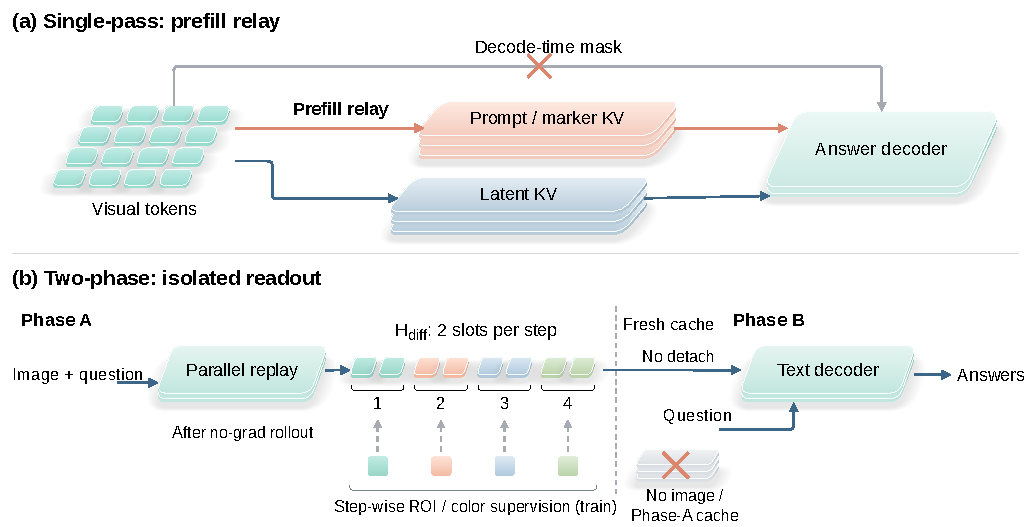
\includegraphics[width=0.78\textwidth]{figs/fig1_teaser_overview.pdf}
  \caption{\textbf{Cached Visual Routes, Across-Layer Interventions, and Isolated Readout.} \textbf{(a)} The image conditions both cache partitions during prefill; a decode-time visual-key mask leaves both cached routes accessible. \textbf{(b)} Each sheet shows KV caches at one layer; dashed columns select the same partition through all $28$ layers. \texttt{C3a/b} and \texttt{C2} are donor swaps on the adapted \texttt{E5} checkpoint (\texttt{C3a} swaps prompt/start caches and recomputes $\Mend$; \texttt{C3b} also transplants $\Mend$'s cache) under visual-key masking at $\Mend$ and answer readout. Rates use eligible subsets; zero flips do not establish image-independent latent caches. \textbf{(c)} Phase A rolls out $H_{\mathrm{raw}}$ without gradients, then uses parallel teacher-forced replay to emit $H_{\mathrm{diff}}$. Following prior isolation principles~\cite{li2026livr,park2026cvrr}, Phase B recomputes all layers from $H_{\mathrm{diff}}$, the question, and markers without image tokens or Phase-A KV, flowing answer-loss gradients through the non-detached tape into replay. Donor swaps interpolate the edited step's two slots ($m=2$, $K=4$ shown).}
  \label{fig:teaser}
\end{figure*}

Recent single-hop studies have scrutinized whether latent states genuinely mediate visual reasoning~\cite{li2026capimagine,guo2026beyond,li2026livr,park2026cvrr,realvr2026}. Perturbations on Monet and Mirage yield minimal single-hop loss~\cite{li2026capimagine}, and decomposing the latent span into slot contents, boundary markers, and format shows that image-conditioned slot contents do not act as portable visual memories when the image remains accessible ($|\text{Normal} - \text{ZeroSlot}| \le 2.7$pp, with marker-only decoding $L=0$ recovering $78\%$--$100\%$ of single-hop gains)~\cite{guo2026beyond}. Architecturally, LIVR~\cite{li2026livr} shows that single-pass learnable bottleneck tokens require masking both prompt-to-vision and answer-to-vision attention in Stage 1, while CVRR~\cite{park2026cvrr} shows that layer-20 multimodal question states retain $99\%$ of single-hop competence ($75.4\%$ vs.\ $75.9\%$ on V*) and that removing original multimodal caches under a strict readout interface (\texttt{w/o Bypass}) collapses six latent reasoners (including \texttt{LVR-7B}) to $35.6\%$. Meanwhile, ReaLVR~\cite{realvr2026} identifies the detached-replay gradient gap in LVR's Stage-2 GRPO and aligns all slots toward a single pooled visual prototype $p^+$.

Building on these single-hop diagnostics and visual-isolation precedents~\cite{guo2026beyond,li2026livr,park2026cvrr}, we investigate \textbf{single- and multi-step relational tracking ($K \in \{1, 2, 4\}$) with explicit autoregressive slot rollouts} across three questions:
(1) \emph{Are native continuous latent slots neutral on distractor-rich relational scenes across $K \in \{1, 2, 4\}$ under intact delimiters?}
(2) \emph{Under step-wise supervision and decoding-time vision masking, how do all-layer latent KV caches ($\KV_H$) versus prefill caches ($\KV_{Q,M}$) mediate predictions?}
(3) \emph{Under a strict image-free interface, what trade-offs govern step-aligned sub-windows, prior calibration, auxiliary supervision, and recurrent slot emission?}

A census of $123,287$ images in COCO~\cite{lin2014coco} shows that natural photos virtually never simultaneously satisfy non-degenerate $K=4$ color transitions and same-color distractor constraints ($M_{\mathrm{dist}} \ge 2$). We construct a controlled benchmark of $50$ dev and $150$ disjoint frozen evaluation clusters, paired with $87$ unseen-color counterfactual pairs ($266$ records), $496$ verified in-vocabulary recoloring records, and $600$ implicit pointer-chaining queries. Across seven modules totaling over $200,000$ passes on \texttt{LVR-7B}~\cite{li2026lvr} and its adapted variants (\cref{fig:teaser}), we establish three contributions:

\textbf{1. Destructive Slot Interference Across $K \in \{1, 2, 4\}$ (\texttt{E3-C}, \texttt{E7-2}).} Across the $150$ frozen clusters, native rollouts degrade $K=2, 4$ chain accuracy by $10.33$--$19.67$pp (\texttt{E3-C}, $9,600$ runs) and already degrade single-hop $K=1$ accuracy on the exact same scenes by $16.00$--$21.67$pp (\texttt{E7-2}, $13,200$ outputs), refuting slot neutrality on distractor-rich scenes. Boundary markers alone are neutral ($\pm 0.67$pp vs.\ \texttt{NoLatent}), whereas zeroing slot inputs (\texttt{Zero-Slot}) recovers $100\%$ of \texttt{NoLatent} accuracy (Proposition~\ref{prop:margin}).

\textbf{2. 28-Layer KV Double Dissociation Under Decoding-Masked Adaptation (\texttt{E3-B}, \texttt{E5}, \texttt{E6-C}).} While single-turn recoloring flips \texttt{LVR-7B} predictions on $61.90\%$--$72.09\%$ of queries ($\|\Delta H\|_2 = 69.25$) and local visual patch swaps (\texttt{E3-B1}) flip $83.93\%$--$93.75\%$ of eligible answers, donor latent patching yields $0.00\%$ flips and flat logit slopes ($\delta M(1) \in [-0.095, -0.011]$, \texttt{E3-B2}). Adapting \texttt{LVR-7B} with step-wise supervision and $60\%$ decoding-time vision masking (\texttt{E5}) raises vision-masked accuracy to $67.00\%$--$85.33\%$ with $0.00\%$ donor flips; 28-layer KV swaps (\texttt{E6-C}, Proposition~\ref{prop:bypass}) show $0.00\%$ flips from $\KV_H$ vs.\ $96.88\%$--$100.00\%$ on eligible pairs from $\KV_{Q,M}$ ($16.46\%$--$40.23\%$ full set), and $-64.00$ to $-73.00$pp under blind prefill.

\textbf{3. Step-Window Control, Prior Trade-Offs, and Recurrent Chaining Under Strict Isolation (\texttt{E6}, \texttt{E7}).} Under a LIVR/CVRR-style image-free interface (Proposition~\ref{prop:isolation}), step-aligned 2-slot windows (\texttt{E6-A}) achieve $82.00\%$--$83.33\%$ ($K=2$) and $72.67\%$--$75.67\%$ ($K=4$) chain accuracy on seen colors ($+63.67$ to $+69.00$pp over shared prototypes \texttt{E6-B}), driven synergistically by ROI-MSE ($38.33\%$--$41.00\%$) and Color-CE ($55.33\%$--$57.33\%$) over \texttt{Answer-CE Only} ($5.00\%$--$5.67\%$, \texttt{E7-3b}). On in-vocabulary recoloring (\texttt{E7-1a}), \texttt{E6-A} achieves $73.40\%/58.53\%$ full-set flips ($+70.19/+58.06$pp window specificity), while $K\times K$ logit matrices (\texttt{E7-3a}) quantify $k=r+1$ spillover (max off-diagonal $0.49$--$0.70$ log-odds). On held-out \texttt{yellow/brown}, narrow training priors limit raw \texttt{E6-A} flips to $0.00\%/3.12\%$, while prior calibration ($23.78\%/45.18\%$) and 8-color+KL training ($85.37\%/82.29\%$ new-color, $57.32\%/47.79\%$ joint flips) unlock unseen colors at a cost to original-image accuracy (\texttt{E7-1b}). Finally, on pointer chaining (\texttt{E7-4}), recurrent emission beats parallel emission by $+10.00$pp in strict readout ($80.67\%$ vs.\ $70.67\%$ on $K=2$; $41.33\%$ vs.\ $31.33\%$ on $K=4$), narrowing the gap to same-weight direct vision ($87.33\%/63.00\%$).

\section{Related Work}
\label{sec:related}

\textbf{Latent Visual Reasoning Paradigms.} Inspired by continuous thought in language models~\cite{hao2025coconut,shen2025codi,goyal2024pause}, recent MLLMs replace verbose textual rationales~\cite{shao2024visualcot} or pixel-cropping tools~\cite{su2025pixelreasoner,zheng2026deepeyes} with continuous latent states. Autoregressive rollout methods such as Mirage~\cite{yang2026mirage}, Latent Sketchpad~\cite{zhang2025sketchpad}, and LVR~\cite{li2026lvr} feed last-layer hidden states between boundary delimiters and supervise them via MSE reconstruction of helper images or ROI patches, while Monet~\cite{wang2026monet} and related variants~\cite{tong2025skila,wang2026laser,jiang2026univlr,cheng2026hylar,adhikari2026pearl} distill teacher trajectories. To move beyond a single initial span, ILVR~\cite{dong2026ilvr} alternates between explicit textual rationales and momentum-aligned latent segments. Conversely, non-autoregressive bottleneck methods discard hidden-state rollouts: LIVR~\cite{li2026livr} appends $K=16$ static learnable vocabulary tokens in a single forward pass with two-stage attention masking, whereas CVRR~\cite{park2026cvrr} eliminates separate latent slots and recurrently refines intermediate multimodal question representations at a fixed decoder layer. Unlike ILVR (which relies on intermediate text) or LIVR and CVRR (which modify token/layer interfaces for single-turn VQA), we examine explicit autoregressive slot spans on multi-step relational queries ($K \in \{2, 4\}$) without intermediate text.

\textbf{Mechanistic Diagnostics and Multi-Step Slot Interference.} On single-hop benchmarks, CapImagine~\cite{li2026capimagine} and concurrent probing studies~\cite{viveiros2026holding,zhang2026cosine,zhang2026unsilencing} observe minimal degradation when latent states are perturbed in Monet and Mirage. Beyond Visual Memory~\cite{guo2026beyond} decomposes the latent span into slot contents, boundary markers, and format across six single-hop settings (MVH, ILVR, Monet), showing that slot contents do not act as portable visual memories when the image is accessible ($|\text{Normal} - \text{ZeroSlot}| \le 2.7$pp while marker-only decoding $L=0$ recovers $78\%$--$100\%$ of single-hop gains), while carefully noting that this does not imply universal slot inertness and documenting self-looping under corrupted markers (\texttt{ZeroMarker}). Extending this decomposition to multi-step queries ($K \in \{2, 4\}$), we show that under intact boundary markers (\texttt{Marker-only} $\approx$ \texttt{NoLatent}), uncalibrated non-zero slots inflict $-10.33$ to $-20.00$pp destructive interference that is $100\%$ eliminated by \texttt{Zero-Slot}, and we reconcile pre-filtered (\texttt{E3-A}) vs.\ unfiltered (\texttt{E3-C}) slot-zeroing behavior via Proposition~\ref{prop:margin}.

\textbf{Visual Isolation Precedents and Multi-Step Sub-Window Control.} Two recent works establish direct architectural precedents for blocking prompt-mediated visual bypasses. In single-pass learnable token training, LIVR~\cite{li2026livr} (Table 6a) shows that masking only answer-to-vision attention fails to improve SFT unless prompt-to-vision attention is simultaneously masked in Stage 1. Complementarily, CVRR~\cite{park2026cvrr} shows that layer-20 multimodal question states (\texttt{Multimodal Q}) in frozen \texttt{Qwen2.5-VL-7B} retain $99\%$ of single-hop visual competence ($75.4\%$ vs.\ $75.9\%$ on V*) and introduces a strict readout interface (\texttt{w/o Bypass}) deleting visual and multimodal prompt caches, under which six latent reasoners (including \texttt{LVR-7B}) collapse to $35.6\%$. Meanwhile, ReaLVR~\cite{realvr2026} identifies the detached-replay gradient gap in LVR's Stage-2 GRPO and aligns all slots toward a single pooled visual prototype $p^+$. Building on the isolation principle of LIVR~\cite{li2026livr} and CVRR~\cite{park2026cvrr}, our experiments (\texttt{E5} and \texttt{E6}) focus on multi-step phenomena and step-wise control: we provide a 28-layer KV-swap double dissociation (\texttt{E6-C}) quantifying how decoding-masked multi-step adaptation routes through $\KV_{Q,M}$ rather than $\KV_H$, show that multi-step isolation requires step-partitioned sub-windows (\texttt{E6-A}) over shared prototypes (\texttt{E6-B}, $+63.7$ to $+69.0$pp), and expose the vocabulary-prior barrier separating conditional logit shifts from discrete out-of-vocabulary counterfactual flips.

\section{Theoretical Framework}
\label{sec:theory}

We establish three exact mathematical propositions on nonlinear causal Transformers without relying on linear-superposition approximations, independent step-wise product assumptions ($p^K$), or degenerate conditional mutual information in deterministic networks. Complete step-by-step proofs are provided in Supplementary Appendix~\ref{app:proofs}.

\subsection{Causal Sequence and Potential Margin Formulation}
\label{subsec:prelim}

Let $\VT \in \mathbb{R}^{M \times d}$ denote the projected visual tokens and $Q \in \mathbb{R}^{T_q \times d}$ denote the prompt tokens. For a $K$-step relational query ($K \in \{2, 4\}$), the model outputs $K$ color predictions $Y = (Y_1, \dots, Y_K) \in \mathcal{A}^K$ with ground-truth labels $Y^* = (y_1^*, \dots, y_K^*)$. With latent reasoning enabled, the sequence follows the causal ordering:
\begin{equation}
  \mathrm{Seq} = \big[\, \VT,\; Q,\; \Mstart,\; H_{1:L},\; \Mend,\; Y_1, \dots, Y_K \,\big],
  \label{eq:seq}
\end{equation}
where $\Mbdy = (\Mstart, \Mend)$ denotes the boundary markers and $H_{1:L} = (h_1, \dots, h_L) \in \mathbb{R}^{L \times d}$ denotes the continuous latent slot inputs.

For step $k \in \{1, \dots, K\}$, let $Y^*_{<k}$ denote the gold prefix and $\hat{Y}_{<k}(m, h)$ denote the greedy prefix under configuration $(m, h)$, where $(\varnothing, \varnothing)$ denotes \texttt{NoLatent}, $(\Mbdy, 0)$ denotes \texttt{Zero-Slot} (or \texttt{Marker-only} when $L=0$), and $(\Mbdy, H)$ denotes \texttt{Native}. Under the chain-rule conditioning event $\{C_1 = 1, \dots, C_{k-1} = 1\}$ of full-chain accuracy (and teacher-forced logit probing), $\hat{Y}_{<k}(m, h) = Y^*_{<k}$. Defining $\mathrm{logit}_k(c \mid \VT, Q, m, h)$ as the step-$k$ output logit for candidate color $c \in \mathcal{A}$, the \textbf{classification margin} of the true label $y_k^*$ is:
\begin{equation}
\begin{aligned}
  M_k(m, h) &\coloneqq \mathrm{logit}_k(y_k^* \mid \VT, Q, m, h) \\
  &\quad - \max_{c \neq y_k^*} \mathrm{logit}_k(c \mid \VT, Q, m, h).
\end{aligned}
\label{eq:margin}
\end{equation}
Under greedy decoding, step-$k$ correctness is the indicator event $C_k(m, h) \coloneqq \mathbb{I}\{M_k(m, h) > 0\} \in \{0, 1\}$.

\subsection{Proposition 1: Telescoping Margin Decomposition and Boundary-Crossing Identity}
\label{subsec:prop1}

Although multilayer Transformers are highly nonlinear, any function admits an exact \textbf{telescoping finite-difference identity} on the same instance $(\VT, Q)$:
\begin{equation}
  M_k(\Mbdy, H) \equiv M_k(\varnothing, \varnothing) + \Delta M_k^{\mathrm{bdy}} + \Delta M_k^{\mathrm{slot}}(H),
  \label{eq:telescope}
\end{equation}
where $\Delta M_k^{\mathrm{bdy}} \coloneqq M_k(\Mbdy, 0) - M_k(\varnothing, \varnothing)$ measures the margin shift from boundary markers alone, and $\Delta M_k^{\mathrm{slot}}(H) \coloneqq M_k(\Mbdy, H) - M_k(\Mbdy, 0)$ measures the shift from non-zero slot vectors $H$ relative to \texttt{Zero-Slot}. Note that $\mathbb{E}[\Delta M_k^{\mathrm{slot}}(H)] < 0$ does not automatically reduce accuracy; accuracy drops if and only if $\Delta M_k^{\mathrm{slot}}(H)$ pushes instances across $M_k = 0$.

\begin{proposition}[Boundary-Crossing Identity, Subset Inclusion, and Multi-Step Telescoping]
\label{prop:margin}
Let $C_k^{(0)} \coloneqq C_k(\Mbdy, 0)$ and $C_k^{(H)} \coloneqq C_k(\Mbdy, H)$. Without linearity or independence assumptions:
\begin{enumerate}
    \item \textbf{Single-Step Boundary-Crossing Identity:} The accuracy difference between \texttt{Zero-Slot} and \texttt{Native} equals the boundary-crossing degradation rate $\pi_k^-$ minus the rescue rate $\pi_k^+$:
    \begin{equation}
      \mathbb{P}(C_k^{(0)} = 1) - \mathbb{P}(C_k^{(H)} = 1) = \pi_k^- - \pi_k^+,
      \label{eq:crossing}
    \end{equation}
    where $\pi_k^- \coloneqq \mathbb{P}(0 < M_k(\Mbdy, 0) \le -\Delta M_k^{\mathrm{slot}}(H))$ is the probability mass in the vulnerable band $(0, -\Delta M_k^{\mathrm{slot}}(H)]$ pulled below zero by non-zero slots, and $\pi_k^+ \coloneqq \mathbb{P}(0 \le -M_k(\Mbdy, 0) < \Delta M_k^{\mathrm{slot}}(H))$.
    \item \textbf{Conditional Subset Inclusion (Reconciling E3-A and E3-C):} On the event $\{\Delta M_k^{\mathrm{slot}}(H) \le 0\}$, any instance succeeding under \texttt{Native} ($M_k(\Mbdy, 0) + \Delta M_k^{\mathrm{slot}}(H) > 0$) automatically satisfies $M_k(\Mbdy, 0) > 0$:
    \begin{equation}
      \mathbb{P}\big(C_k^{(0)} = 1 \;\big|\; C_k^{(H)} = 1,\; \Delta M_k^{\mathrm{slot}}(H) \le 0\big) \equiv 1.
      \label{eq:subset_inclusion}
    \end{equation}
    Hence zeroing slots on pre-filtered subsets where $C_k^{(H)}=1$ (\texttt{E3-A}) preserves predictions with probability near $1$, whereas on the unfiltered population (\texttt{E3-C}) it rescues the entire vulnerable mass $\pi_k^- > 0$.
    \item \textbf{Multi-Step Product Telescoping:} For full-chain accuracy $\mathrm{Acc}_{\mathrm{joint}}(K) = \mathbb{E}[\prod_{k=1}^K C_k]$ under arbitrary within-scene correlation $\mathrm{Cov}(C_j, C_k) > 0$:
    \begin{equation}
    \begin{aligned}
      &\mathrm{Acc}_{\mathrm{joint}}^{(0)}(K) - \mathrm{Acc}_{\mathrm{joint}}^{(H)}(K) \\
      &\equiv \sum_{k=1}^K \mathbb{E}\!\left[ \Big(\prod_{j<k} C_j^{(0)}\Big) \big(C_k^{(0)} - C_k^{(H)}\big) \Big(\prod_{m>k} C_m^{(H)}\Big) \right]\!,
    \end{aligned}
    \label{eq:multistep_telescope}
    \end{equation}
    and the joint error rate satisfies the Fr\'echet bounds $\max_k e_k \le 1 - \mathrm{Acc}_{\mathrm{joint}}(K) \le \min(1, \sum_{k=1}^K e_k)$, where $e_k = 1 - \mathbb{E}[C_k]$.
\end{enumerate}
\end{proposition}

\textbf{Counterfactual Margin Shift.} For a counterfactual pair $(\Vorig, \Vrel)$ where target step $m$'s color changes from $a_m$ to $a_m'$, let $H(\alpha) = (1-\alpha)H(\Vorig) + \alpha H(\Vrel)$. We define the relative log-odds shift on fixed recipient context $\Vorig$ as:
\begin{equation}
\begin{aligned}
  \delta M_m(\alpha) &\coloneqq \big[\mathrm{logit}_m(a_m' \mid \Vorig, H(\alpha)) \\
  &\quad - \mathrm{logit}_m(a_m \mid \Vorig, H(\alpha))\big] - M_m(0),
\end{aligned}
\label{eq:delta_m}
\end{equation}
where $M_m(0)$ is the baseline relative log-odds on $\Vorig$. Greedy output flips from $a_m$ to $a_m'$ only when $\delta M_m(\alpha) > -M_m(0)$.

\subsection{Proposition 2: Prefill KV Relay Confounding and Causal Separation}
\label{subsec:prop2}

In a deterministic network where $H = f_\theta(\VT, Q)$, conditional entropy $H(H \mid \VT, Q) = 0$, so statistical conditional mutual information $I(Y; H \mid \VT, Q) \equiv 0$ regardless of causal reliance. We therefore formulate pathway separation via structural causal models (SCMs)~\cite{geiger2021causal}.

\begin{proposition}[Prefill KV Relay Confounding and Double Dissociation Criterion]
\label{prop:bypass}
In a $D$-layer ($D \ge 2$) causal Transformer on $\mathrm{Seq} = [\VT, Q, \Mstart, H_{1:L}, \Mend, Y]$, answer decoding is governed by three KV-cache groups:
\begin{equation}
  Y = g_\theta\big(\, m_{\mathrm{vis}} \odot \KV_V(\VT),\; \KV_{Q,M}(\VT, Q),\; \KV_H(H_{1:L}) \,\big),
  \label{eq:scm}
\end{equation}
where $m_{\mathrm{vis}} \in \{0, 1\}$ controls answer-to-vision attention and $\KV_{Q,M}$ denotes non-visual prompt/marker caches.
\begin{enumerate}
    \item \textbf{Prefill Visual Relay ($P_2$):} Because $Q$ and $\Mstart$ follow $\VT$ in $\mathrm{Seq}$, layer-1 self-attention computes $h_Q^{(1)}$ from $\VT$, making $\KV_{Q,M}^{(\ell)}(\VT, Q)$ an entangled function of $(\VT, Q)$ for all layers $\ell \ge 2$. Setting $m_{\mathrm{vis}} = 0$ (\texttt{Vision-Masked} decoding) blocks only the direct path $P_1$ ($\VT \to \KV_V \to Y$), leaving open both the prefill relay $P_2$ ($\VT \to \KV_{Q,M}(\VT, Q) \to Y$) and the latent path $P_3$ ($\VT \to \KV_H \to Y$).
    \item \textbf{Identification via Double Dissociation:} Under $m_{\mathrm{vis}} = 0$, let $\tau_{\mathrm{lat}}(0)$ be the target flip rate under $\Do(\KV_H \leftarrow \KV_H(\Vrel))$ with $\KV_{Q,M}(\Vorig, Q)$ fixed, $\tau_{\mathrm{relay}}(0)$ be the flip rate under $\Do(\KV_{Q,M} \leftarrow \KV_{Q,M}(\Vrel, Q))$ with $\KV_H(\Vorig)$ fixed, and $\Delta_{\mathrm{zero}}(0)$ be the accuracy drop under $\Do(H_{1:L} \leftarrow 0)$. If $\mathbb{P}(Y_{\mathrm{mask}} = Y^*) \gg 0$ while $\tau_{\mathrm{lat}}(0) = 0$, $\Delta_{\mathrm{zero}}(0) \le 0$, and $\tau_{\mathrm{relay}}(0) \approx \tau_{\mathrm{total}}(0)$, visual competence under $m_{\mathrm{vis}}=0$ is routed exclusively via $P_2$ ($\KV_{Q,M}$). Notably, $\Delta_{\mathrm{zero}}(0) \le 0$ rules out even nonlinear AND-gate interactions between $P_2$ and $P_3$, since $g_\theta(0, \KV_{Q,M}(\VT, Q), 0)$ retains full cross-image discriminability with its third argument fixed to $0$.
\end{enumerate}
\end{proposition}

\subsection{Proposition 3: Exact Equivalence Under Full Prefill-and-Decode Visual Isolation}
\label{subsec:prop3}

\begin{proposition}[Exact Counterfactual Equivalence Under Full Visual Isolation]
\label{prop:isolation}
Suppose answer decoding satisfies \textbf{Full Prefill-and-Decode Visual Isolation}:
(i) direct visual attention is blocked ($m_{\mathrm{vis}} = 0$);
(ii) non-latent text/marker caches visible to the decoder are strictly image-free, $\KV_{Q,M}(\Vorig, Q) = \KV_{Q,M}(\Vrel, Q) = \KV_{Q,M}(Q)$ (e.g., decoding from $\mathrm{Seq}_B = [Q, \Mstart, H_{1:L}, \Mend, Y]$ without $\VT$ or Phase-A caches); and
(iii) donor intervention substitutes $H_{1:L} \leftarrow H(\Vrel, Q)$ without re-attending to $\Vorig$.
Then for any model $g_\theta$ and any same-question pair $(\Vorig, \Vrel)$, the donor-intervened output on $\Vorig$ is sample-by-sample identical to the direct output on $\Vrel$:
\begin{equation}
\begin{aligned}
  &Y\big(\Vorig, Q, \Do(H \leftarrow H(\Vrel, Q))\big) \\
  &= g_\theta\big(0,\, \KV_{Q,M}(Q),\, \KV_H(H(\Vrel, Q))\big) \equiv Y(\Vrel, Q),
\end{aligned}
\label{eq:exact_equiv}
\end{equation}
guaranteeing exact equality between latent-mediated and total input counterfactual effects: $\tau_{\mathrm{lat}} \equiv \tau_{\mathrm{total}}(\Vorig \to \Vrel)$.
\end{proposition}

\section{Controlled Multi-Step Benchmark \& Method}
\label{sec:benchmark}

\textbf{123K-Image COCO Census and Frozen Benchmark.}
\label{subsec:census}
Testing Propositions~\ref{prop:margin}--\ref{prop:isolation} requires eliminating two shortcuts pervasive in natural VQA datasets~\cite{hudson2019gqa,lin2014coco}: (a) \emph{monochrome repetition}, where target objects share the same color ($46\%$ of GQA dev scenes and $50\%$ of candidates), and (b) \emph{missing same-color distractors}, which allows global perception to bypass relational hops. A programmatic census of all $123,287$ images in COCO~\cite{lin2014coco} (excluding $297$ grayscale photos) revealed that requiring $K=4$ non-overlapping targets with non-degenerate color transitions and $M_{\mathrm{dist}} \ge 2$ disjoint same-color, same-category distractors per target yields \textbf{zero ($0 / 123,287$)} qualifying natural images among $300$ geometric candidates. We therefore constructed a frozen controlled benchmark from COCO instances with strict train-test separation:
(1) \textbf{Disjoint Dev and Frozen Eval Splits ($K \in \{1, 2, 4\}$):} We built $150$ frozen evaluation clusters ($92$ instance-composited and $58$ polygon-recolored scenes from $1,070$ source photos) and $50$ disjoint dev clusters ($40$ train, $10$ val from $400$ source photos with \textbf{zero source-image overlap}), enforcing $M_{\mathrm{dist}} \ge 2$ same-color distractors and non-degenerate target colors (\texttt{red, green, blue}). Dev-calibrated position permutation matching balances single-hop \texttt{NoLatent} accuracy across positions $1$--$4$ within $4.67$pp ($76.67\%$--$81.33\%$). Each cluster is evaluated across $4$ multi-step conditions ($K \in \{2, 4\} \times \{\text{Indep.}, \text{Serial}\}$) and $2$ templates ($1,200$ queries/strategy), plus $600$ single-hop $K=1$ queries (\texttt{E7-2}) and $600$ implicit pointer-chaining queries (\texttt{E7-4}, where step $k$ is defined relative to $O_{k-1}$ from anchor $O_1$).
(2) \textbf{Unseen-Color and In-Vocabulary Counterfactuals:} Across $64$ clusters, we created $87$ pixel-level counterfactual triplets $(\Vorig, \Vrel, \Virrel)$ ($266$ records: $92$ for $K=2$ / $41$ clusters; $174$ for $K=4$ / $64$ clusters) rotating the step-$m$ target mask from \texttt{red/green} to held-out \texttt{yellow} ($176$) or \texttt{brown} ($90$). To decouple sub-window control from vocabulary priors (\texttt{E7-1a}), we also constructed $496$ verified \textbf{in-vocabulary recoloring records} across $62$ clusters ($176$ for $K=2$ / $39$ clusters; $320$ for $K=4$ / $62$ clusters, $\ge 0.80$ crop confidence) rotating strictly within \texttt{red $\leftrightarrow$ green $\leftrightarrow$ blue}.

\textbf{Two-Phase Strict Isolation Interface (\texttt{E6} \& \texttt{E7}).}
\label{subsec:method_e6}
All experiments evaluate official \texttt{LVR-Qwen2.5-VL-7B-SFT}~\cite{li2026lvr} and \texttt{Qwen2.5-VL-7B-Instruct}~\cite{bai2025qwen25vl} under greedy decoding ($\text{temperature}=0$). Following the visual-isolation principles of LIVR~\cite{li2026livr} and CVRR~\cite{park2026cvrr}, our \textbf{Two-Phase Strict Isolation Interface} (\cref{fig:teaser}c) comprises:
(1) \textbf{Phase A (Parallel vs.\ Recurrent Emission):} Given $[\VT, Q, \Mstart]$, we roll out $L = 2K$ states $H_{1:L}^{\mathrm{raw}}$ under \texttt{torch.no\_grad()}. In \textbf{Parallel Phase A (\texttt{E6-A})}, a single teacher-forced pass on $[\VT, Q, \Mstart, H_{1:L}^{\mathrm{raw}}]$ emits $H_{\mathrm{diff}} \in \mathbb{R}^{L \times d}$, supervising each 2-slot window $H_{\mathrm{diff}}^{(k)}$ with normalized ROI MSE $\mathcal{L}_{\mathrm{ROI}}^{(k)}$ against target box $b_k^*$ plus $0.1\times$ 8-color CE $\mathcal{L}_{\mathrm{color}}^{(k)}$ (ablated in \texttt{E7-3b}). In \textbf{Recurrent Phase A (\texttt{E7-4})}, window $k$ causally attends to window $(k{-}1)$'s differentiable output without \texttt{detach}.
(2) \textbf{Phase B (Strict Image-Free Readout):} We feed $H_{\mathrm{diff}}$ into a newly initialized pure-text sequence $\mathrm{Seq}_B = [Q,\, \Mstart,\, H_{\mathrm{diff}},\, \Mend,\, Y]$ with \textbf{zero image tokens and zero Phase-A KV caches}, backpropagating $\nabla_{H_{\mathrm{diff}}} \mathcal{L}_{\mathrm{ans}}$ into Phase-A LoRA weights (\texttt{q/k/v/o\_proj}, rank $16$, $\alpha=32$). Shared-prototype \textbf{\texttt{E6-B}}~\cite{realvr2026} supervises all $2K$ slots with the union-pooled ROI feature and color distribution of all $K$ targets.

\section{Experiments and Mechanistic Analysis}
\label{sec:experiments}

We conduct a causal audit across seven experimental modules (\texttt{Pilot}, \texttt{E1}, \texttt{E2-A}, \texttt{E3-A/B/C}, \texttt{E5}, \texttt{E6}, and \texttt{E7}), totaling over $200,000$ forward and intervention passes. All bracketed confidence intervals represent $5,000$-iteration scene-cluster bootstrap $95\%$ intervals, averaging templates and edits within each source scene cluster before resampling.

\subsection{Destructive Slot Interference Across $K \in \{1, 2, 4\}$ (\texttt{Pilot}, \texttt{E1}, \texttt{E3-C}, \texttt{E7-2})}
\label{subsec:exp_e3c}

\textbf{Single-Hop Public Benchmarks (\texttt{Pilot}).} Across $991$ public single-hop examples in TreeBench~\cite{treebench2025} ($400$), HR-Bench 4K/8K~\cite{wang2024hrbench} ($400$), and V*Bench~\cite{wu2024vstar} ($191$), native \texttt{LVR-7B} ($L \in \{4, 8, 16\}$) achieves $48.51\%$--$48.81\%$ weighted accuracy, matching \texttt{NoLatent} ($48.76\%$), slot zeroing ($H \leftarrow 0$, $48.81\%$), and Gaussian noise ($48.56\%$), whereas decoding-time \texttt{Vision-Mask} drops accuracy to $28.61\%$ (Supplementary Table~S1), consistent with single-hop non-portability~\cite{guo2026beyond}.

\begin{table*}[!t]
  \caption{\textbf{Same-Scene Single- and Multi-Step Component Dissociation on 150 Frozen Scene Clusters (\texttt{E3-C} $9,600$ Runs \& \texttt{E7-2} $13,200$ Outputs).} Left: $K=1$ single-hop accuracy on Template 0 ($600$ queries/arm, \texttt{E7-2}). Middle \& Right: $K \in \{2, 4\}$ full-chain exact-match accuracy ($\%$) and $K=4$ per-position mean ($\%$) / slope (pp/step) across both templates (\texttt{E3-C}). Boundary markers (\texttt{Marker-only}) are neutral ($\pm 0.67$pp), whereas native non-zero slots induce $-16.00$ to $-21.67$pp single-hop and $-10.33$ to $-20.00$pp multi-step degradation, $100\%$ recovered by \texttt{Zero-Slot}.}
  \label{tab:e3c}
  \centering
  \resizebox{\textwidth}{!}{%
  \begin{tabular}{l c c c c c c c}
    \toprule
    & \textbf{$K=1$ Single-Hop} & \multicolumn{4}{c}{\textbf{Multi-Step Full-Chain Exact-Match Accuracy (\texttt{E3-C}, \%)}} & \multicolumn{2}{c}{\textbf{$K=4$ Position Mean (\%) / Slope}} \\
    \cmidrule(lr){2-2} \cmidrule(lr){3-6} \cmidrule(lr){7-8}
    \textbf{Strategy / Intervention Arm} & \textbf{(\texttt{E7-2} T0, \%)} & \textbf{$K=2$ Indep.} & \textbf{$K=2$ Serial} & \textbf{$K=4$ Indep.} & \textbf{$K=4$ Serial} & \textbf{$K=4$ Indep.} & \textbf{$K=4$ Serial} \\
    \midrule
    \texttt{NoLatent} & $83.33\ci{80.50}{86.17}$ & $76.00\ci{70.00}{82.33}$ & $\mathbf{73.67}\ci{66.67}{80.33}$ & $30.67\ci{24.00}{37.67}$ & $35.00\ci{27.67}{42.00}$ & $68.67 / {-6.53}$ & $71.50 / {-5.33}$ \\
    \texttt{Marker-only} ($L=0$) & $83.50\ci{80.50}{86.33}$ & $76.33\ci{70.00}{82.33}$ & $73.33\ci{66.66}{79.67}$ & $31.33\ci{24.33}{38.33}$ & $34.33\ci{27.00}{41.67}$ & $68.58 / {-6.03}$ & $70.42 / {-4.77}$ \\
    \texttt{Native} $L=4$ ($L=2$: $67.33\%$ on $K{=}1$) & $63.33\ci{58.83}{67.67}$ & $64.00\ci{57.00}{70.67}$ & $63.00\ci{56.33}{69.67}$ & $18.00\ci{13.00}{23.33}$ & $21.00\ci{15.33}{27.00}$ & $58.58 / {-3.83}$ & $61.33 / {-2.07}$ \\
    \texttt{Native} $L=8$ & $61.67\ci{57.33}{66.00}$ & $56.33\ci{49.00}{63.34}$ & $57.00\ci{49.67}{64.00}$ & $19.00\ci{13.67}{24.33}$ & $24.33\ci{18.67}{30.33}$ & $61.00 / {-2.80}$ & $63.92 / {-1.10}$ \\
    \rowcolor{resulttint}
    \texttt{Zero-Slot} $L=4$ & $\mathbf{83.67}\ci{80.83}{86.50}$ & $\mathbf{77.00}\ci{71.00}{83.00}$ & $73.33\ci{66.33}{79.67}$ & $32.67\ci{25.67}{39.67}$ & $\mathbf{36.33}\ci{29.33}{43.67}$ & $\mathbf{68.83} / {-7.00}$ & $\mathbf{72.08} / {-5.77}$ \\
    \rowcolor{resulttint}
    \texttt{Zero-Slot} $L=8$ & $\mathbf{83.67}\ci{80.83}{86.33}$ & $76.33\ci{70.00}{82.33}$ & $72.33\ci{65.67}{79.00}$ & $\mathbf{33.33}\ci{26.33}{40.33}$ & $\mathbf{36.33}\ci{29.00}{43.67}$ & $68.67 / {-7.53}$ & $72.00 / {-6.93}$ \\
    \texttt{Zero-Marker} $L=4$ & $62.83\ci{58.33}{67.33}$ & $64.33\ci{57.33}{71.33}$ & $62.67\ci{55.67}{69.33}$ & $19.00\ci{14.00}{24.00}$ & $21.00\ci{15.67}{26.67}$ & $59.00 / {-3.87}$ & $61.83 / {-2.27}$ \\
    \texttt{Zero-Marker} $L=8$ & $61.83\ci{57.50}{66.17}$ & $56.33\ci{49.33}{63.33}$ & $57.00\ci{50.00}{64.00}$ & $19.67\ci{14.33}{25.00}$ & $25.33\ci{19.33}{31.67}$ & $61.92 / {-3.37}$ & $65.00 / {-0.73}$ \\
    \midrule
    \texttt{Marker-only} $-$ \texttt{NoLatent} & $+0.17\ci{-0.50}{1.00}$ & $+0.33\ci{0.00}{1.00}$ & $-0.33\ci{-2.00}{1.33}$ & $+0.67\ci{-0.67}{2.00}$ & $-0.67\ci{-2.00}{0.67}$ & \multicolumn{2}{c}{Markers neutral; \texttt{Zero-Slot} $L{=}8{-}\text{Nat}{=}+12.0\text{--}22.0$pp} \\
    \texttt{Zero-Slot} $-$ \texttt{Native} ($L=4$) & $\mathbf{+20.33}\ci{16.17}{24.83}$ & $\mathbf{+13.00}\ci{6.67}{19.33}$ & $\mathbf{+10.33}\ci{4.00}{16.67}$ & $\mathbf{+14.67}\ci{8.67}{20.67}$ & $\mathbf{+15.33}\ci{10.00}{20.67}$ & \multicolumn{2}{c}{$100\%$ recovery via slot zeroing} \\
    \bottomrule
  \end{tabular}%
  }
\end{table*}

\begin{figure}[!t]
  \centering
  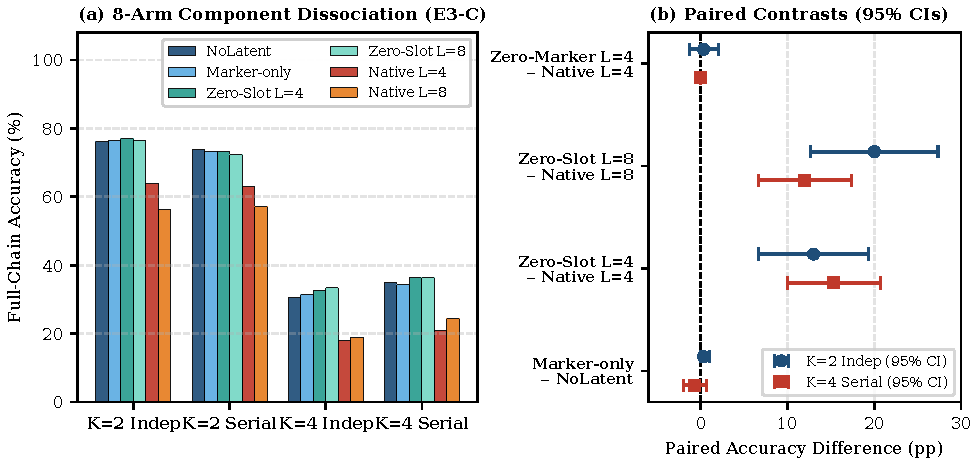
\includegraphics[width=\linewidth]{figs/fig2_e3c_slot_interference.pdf}
  \caption{\textbf{Destructive Slot Interference Across $K \in \{1, 2, 4\}$ (\texttt{E3-C} \& \texttt{E7-2}).} \textbf{(a)} Same-scene accuracy on 150 frozen clusters ($K=1$ on Template 0; $K=2, 4$ full-chain across both templates). \textbf{(b)} Paired cluster-bootstrap differences ($95\%$ CI, $L=4$): boundary markers are neutral ($\pm 0.67$pp), whereas \texttt{Zero-Slot} minus \texttt{Native} yields $+20.33$pp on $K=1$ and $+10.33$--$15.33$pp on $K=2, 4$ ($+20.00$pp at $L=8$).}
  \label{fig:e3c}
\end{figure}

\textbf{Same-Scene $K \in \{1, 2, 4\}$ Component Dissociation (\texttt{E1}, \texttt{E3-C}, \texttt{E7-2}).} Across the $150$ frozen clusters (\cref{tab:e3c}, \cref{fig:e3c}, and Supplementary Table~S14), native rollouts cause severe negative transfer across both single- and multi-step queries. On $K=2, 4$ (\texttt{E3-C}, $9,600$ runs), \texttt{NoLatent} $K=4$ independent and serial chain accuracies are $30.67\%$ and $35.00\%$ (serial position mean $\bar{p}=71.50\%$ exceeds $\bar{p}^4 = 26.13\%$ due to within-scene correlation $\mathrm{Cov}(C_j, C_k) > 0$, Proposition~\ref{prop:margin}; serial-vs-independent interaction $I_{\mathrm{fixed}} = -2.67\ci{-9.33}{4.00}$pp spans zero). Native rollouts ($L=4, 8$) lower per-position accuracy by $\pi_k^- - \pi_k^+ \approx 10.1$pp ($71.50\% \to 61.33\%$ on $K=4$ serial), compounding via Eq.~\eqref{eq:multistep_telescope} into a $10.33$--$20.00$pp full-chain drop ($35.00\% \to 21.00\%$ on $K=4$ serial; $76.00\% \to 56.33\%$ on $K=2$ indep.\ $L=8$).
Evaluating all $11$ arms ($L \in \{2, 4, 8\}$) on single-hop $K=1$ queries on the \emph{exact same 150 scenes} (\texttt{E7-2}, $13,200$ outputs) shows that \texttt{Native} $L=2/4/8$ already drops $K=1$ accuracy from $83.33\%$ (\texttt{NoLatent}) to $67.33\% / 63.33\% / 61.67\%$ ($\mathbf{-16.00}$\textbf{, }$\mathbf{-20.00}$\textbf{, and }$\mathbf{-21.67}$\textbf{pp}), whereas \texttt{Marker-only} ($83.50\%$) and \texttt{Zero-Slot} ($83.67\%$) restore $100\%$ of \texttt{NoLatent} accuracy. Thus, destructive slot interference is \emph{not} exclusive to multi-step tracking: by Proposition~\ref{prop:margin}, same-color distractors place baseline margins near $M_k=0$, exposing negative slot shifts $\Delta M_k^{\mathrm{slot}}(H) < 0$ even at $K=1$ ($K=1$ \texttt{NoLatent} $83.33\%$ is slightly below $K=2$ independent per-position $88.00\%$ on Template 0 due to prompt/length differences).

\subsection{Input Sensitivity vs.\ Zero Readout (\texttt{E2-A}, \texttt{E3-A/B})}
\label{subsec:exp_e3b}

\textbf{Input Sensitivity (\texttt{E2-A}) vs.\ Donor Swap (\texttt{E3-A}).} Across the $87$ counterfactual pairs ($3,192$ \texttt{E2-A} runs), recoloring the step-$m$ target ($\Vrel$) flips native \texttt{LVR-7B} predictions on $61.90\%$--$72.09\%$ of pairs ($0.00\%$ false flips on $\Virrel$) and shifts $H$ by $\|\Delta H\|_2 = 69.25$ (Supplementary Table~S2). Yet across $15,484$ \texttt{E3-A} runs ($384$ doubly eligible injections), patching $H(\Vrel)$ into $\Vorig$ yields \textbf{$0.00\%$} target flips (Supplementary Table~S3), while \texttt{Zero-Patch} on this pre-filtered $C_k^{(H)}=1$ subset retains the original answer on $95.35\%$--$98.86\%$ of instances, matching Proposition~\ref{prop:margin}.

\begin{table}[!t]
  \caption{\textbf{Local Visual Patch Swap Positive Control vs.\ ROI-Masked Latent Injection (\texttt{E3-B1}) and Logit Shift (\texttt{E3-B2}, $19,152$ Runs).} Target-step net directional transfer (pp) on Full / Position-Eligible / Chain-Eligible subsets, and full-set conditional log-odds shift $\delta M(1)$ (Unmasked / Vision-Masked).}
  \label{tab:e3b}
  \centering
  \resizebox{\linewidth}{!}{%
  \begin{tabular}{l c c c}
    \toprule
    \textbf{Cond.} & \textbf{Pos.\ Control: Visual Patch} & \textbf{ROI-Masked Latent} & \textbf{Logit Shift $\delta M(1)$} \\
    $(K, L)$ & \textbf{Swap (Full / Pos / Chain)} & \textbf{Swap (Full / Pos / Chain)} & \textbf{(Unmask / V-Mask)} \\
    \midrule
    $(2, 4)$  & $+48.8 / \mathbf{+83.9} / \mathbf{+85.4}$ & $-1.2 / \phantom{+}0.0 / +2.1$ & $-0.068 / {-0.070}$ \\
    $(2, 8)$  & $+50.0 / \mathbf{+87.0} / \mathbf{+91.3}$ & $-2.4 / \phantom{+}0.0 / \phantom{+}0.0$ & $-0.092 / {-0.072}$ \\
    $(2, 16)$ & $+53.7 / \mathbf{+93.5} / \mathbf{+93.8}$ & $-2.4 / \phantom{+}0.0 / \phantom{+}0.0$ & $-0.095 / {-0.060}$ \\
    $(4, 4)$  & $+42.7 / \mathbf{+87.6} / \mathbf{+89.8}$ & $+0.5 / +2.6 / \mathbf{\phantom{+}0.0}$ & $-0.016 / {-0.012}$ \\
    $(4, 8)$  & $+46.7 / \mathbf{+90.5} / \mathbf{+91.9}$ & $-0.7 / {-0.8} / \mathbf{\phantom{+}0.0}$ & $-0.015 / {-0.011}$ \\
    $(4, 16)$ & $+49.4 / \mathbf{+85.5} / \mathbf{+86.7}$ & $-0.8 / {-1.3} / \mathbf{\phantom{+}0.0}$ & $-0.026 / {-0.021}$ \\
    \bottomrule
  \end{tabular}%
  }
\end{table}

\textbf{Positive Control (\texttt{E3-B1}) and Logit Probing (\texttt{E3-B2}).} Across $19,152$ runs on the $266$ paired records (\cref{tab:e3b}), keeping $H(\Vorig)$ fixed and replacing only the visual tokens inside the target bounding box (\texttt{Visual Patch Swap}) flips \textbf{$83.93\%$--$93.75\%$} of eligible instances ($42.71\%$--$53.66\%$ full set). Conversely, masking those target-ROI visual keys during text decoding and injecting $H(\Vrel)$ yields near-zero net transfer ($-2.44$pp to $+2.56$pp), and 8-point interpolation $\alpha \in [0, 2]$ (\texttt{E3-B2}) yields flat/negative shifts across all $12$ conditions ($\delta M(1) \in [-0.0949, -0.0109]$; \cref{fig:logit_curves}).

\subsection{Decoding-Masked Adaptation and 28-Layer KV Double Dissociation (\texttt{E5} \& \texttt{E6-C})}
\label{subsec:exp_e5_e6c}

\textbf{Eliminating Interference Without Awakening Slots (\texttt{E5}).} Adapting \texttt{LVR-7B} on the $40$ dev training clusters ($2$ epochs, $160$ updates) with step-wise ROI alignment, $0.1\times$ 8-color CE, and $60\%$ decoding-time vision masking ($m_{\mathrm{vis}}=0$, $\mathrm{TBPTT}=1$) eliminates slot interference on the $150$ clusters ($K=4$ serial jumps by $\mathbf{+49.00}$\textbf{pp} to $70.00\%$; $K=4$ independent by $\mathbf{+51.67}$\textbf{pp} to $70.67\%$, matching adapted \texttt{NoLatent} at $70.00\%$), while \texttt{Vision-Masked} accuracy surges from ${\sim}3\%$ to \textbf{$82.33\%$--$85.33\%$} ($K=2$) and \textbf{$67.00\%$--$69.67\%$} ($K=4$; Supplementary Table~S7). Yet across $20,482$ post-adaptation \texttt{E3-A} runs, donor latent transfer under both unmasked and \texttt{Vision-Masked} decoding remains \textbf{$0.00\%\ci{0.00}{0.00}$} (Supplementary Table~S6).

\begin{table}[!t]
  \caption{\textbf{28-Layer KV-Cache Double Dissociation on the \texttt{E5} Checkpoint Under \texttt{Vision-Masked} Decoding (\texttt{E6-C}).} Target-position flip rates ($\%$) across $266$ counterfactual records. Swapping 28-layer latent caches ($\KV_H$, Arm C2) yields $0.00\%$ flips, whereas swapping prefill prompt/marker caches ($\KV_{Q,M}$, Arms C3a/b) yields $96.88\%$--$100.00\%$ flips on eligible subsets ($16.46\%$--$40.23\%$ full set). Blinding prefill caches (Arm C4) on the 150 clusters drops masked accuracy by $64.00$--$73.00$pp.}
  \label{tab:e6c}
  \centering
  \resizebox{\linewidth}{!}{%
  \begin{tabular}{l c c c c c}
    \toprule
    \textbf{Subset / Task} & \textbf{C1: Tape} & \textbf{C2: 28-L} & \textbf{C3a: Prompt} & \textbf{C3b: All Text} & \textbf{All-Vis.} \\
    (Records / Clusters) & $H$ \textbf{Swap} & $\KV_H$ \textbf{Swap} & $\KV_{Q,\mathrm{start}}$ & $\KV_{Q,\mathrm{mkr}}$ & \textbf{Donor Ref.} \\
    \midrule
    $K=2$ Full ($92/41$)    & $0.00$ & $0.00$ & $\mathbf{16.46}$ & $\mathbf{16.46}$ & $16.46$ \\
    \rowcolor{resulttint}
    $K=2$ Pos/Chn ($17/9$)  & $0.00$ & $0.00$ & $\mathbf{100.00}$ & $\mathbf{100.00}$ & $100.00$ \\
    $K=4$ Full ($174/64$)   & $0.00$ & $0.00$ & $\mathbf{40.23}$ & $39.19$ & $39.58$ \\
    \rowcolor{resulttint}
    $K=4$ Pos.\ ($73/32$)   & $0.00$ & $0.00$ & $\mathbf{96.88}$ & $\mathbf{96.88}$ & $100.00$ \\
    \rowcolor{resulttint}
    $K=4$ Chain ($63/27$)   & $0.00$ & $0.00$ & $\mathbf{100.00}$ & $\mathbf{100.00}$ & $100.00$ \\
    \midrule
    \multicolumn{6}{l}{\textbf{C4 Blind Prefill (150 Clust.):} $K{=}2$ S/I $\mathbf{-72.0 / {-73.0}\text{pp}}$; $K{=}4$ S/I $\mathbf{-66.3 / {-64.0}\text{pp}}$} \\
    \bottomrule
  \end{tabular}%
  }
\end{table}

\begin{figure}[!t]
  \centering
  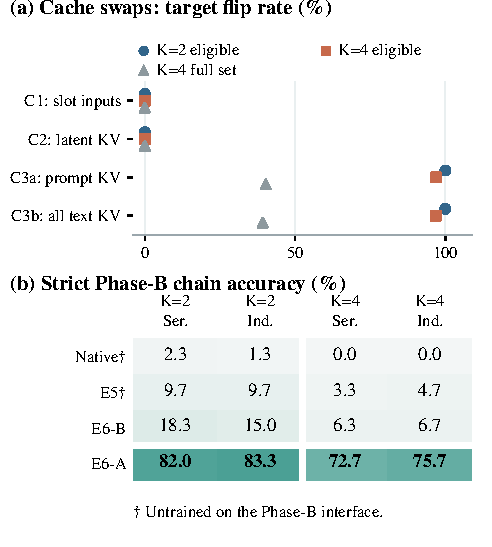
\includegraphics[width=\linewidth]{figs/fig3_e6c_double_dissociation.pdf}
  \caption{\textbf{Cache-Level Double Dissociation (\texttt{E6-C}) and Strict Phase-B In-Domain Accuracy (\texttt{E6-2} \& \texttt{E7-3b}).} \textbf{(a)} Under \texttt{E5} \texttt{Vision-Masked} decoding, swapping 28-layer $\KV_H$ caches yields $0.0\%$ flips, whereas swapping prefill $\KV_{Q,M}$ caches flips $96.9\%$--$100.0\%$ of eligible pairs ($40.2\%$ full set). \textbf{(b)} Under strict image-free Phase B on the 150 frozen clusters, step-aligned sub-windows (\texttt{E6-A}) achieve $72.7\%$--$83.3\%$ chain accuracy ($+63.7$ to $+69.0$pp over shared-prototype \texttt{E6-B}), driven synergistically by spatial ROI-MSE and color supervision.}
  \label{fig:e6c}
\end{figure}

\begin{figure*}[!t]
  \centering
  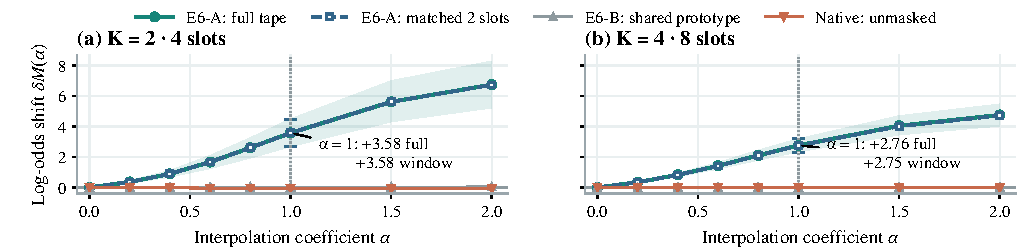
\includegraphics[width=\textwidth]{figs/fig4_e6_logit_interpolation.pdf}
  \caption{\textbf{Conditional Interpolation Logit Shift $\delta M(\alpha)$ Across All 266 Counterfactual Pairs (\texttt{E6-4e} vs.\ \texttt{E3-B2}).} Native \texttt{LVR-7B} and shared-prototype \texttt{E6-B} remain flat near zero, whereas \texttt{E6-A} drives a monotonic positive conditional log-odds shift ($+3.58$ on $K=2$, $+2.76$ on $K=4$ at $\alpha=1$). Interpolating \emph{only the 2 slots of the edited step} (dashed navy) matches the full-tape shift on the edited step ($+3.58$ on $K=2$, $+2.75$ on $K=4$). Both panels share the same vertical scale; shading shows full-tape $95\%$ cluster-bootstrap intervals and error bars at $\alpha=1$ show matched-window intervals.}
  \label{fig:logit_curves}
\end{figure*}

\textbf{28-Layer KV Double Dissociation (\texttt{E6-C}).} Because zeroing input vectors $H_{1:L} \leftarrow 0$ does not stop slot positions from attending to $\VT$ across layers (Proposition~\ref{prop:bypass}), we run four cache-level arms on \texttt{E5} under unified post-$\Mend$ \texttt{Vision-Masked} readout (\cref{tab:e6c} and \cref{fig:e6c}a): swapping all 28 layers of $\KV_H$ (\texttt{Arm C2}) yields \textbf{$0.00\%$} flips, whereas holding $\KV_H(\Vorig)$ fixed and swapping prefill caches $\KV_{Q,\mathrm{start}}(\Vrel)$ (\texttt{Arm C3a}) or $\KV_{Q,\mathrm{mkr}}(\Vrel)$ (\texttt{Arm C3b}) flips \textbf{$100.00\%$} of $K=2$ and $K=4$ chain-eligible pairs ($96.88\%$ position-eligible; $16.46\%$ and $39.19\%$--$40.23\%$ full set, matching the $16.46\%$ and $39.58\%$ all-visible donor reference). Feeding a black image to prefill $\KV_{Q,M}$ while keeping the real image's 28-layer $\KV_H(\VT)$ (\texttt{Arm C4}) drops \texttt{Vision-Masked} accuracy on the $150$ clusters by $\mathbf{64.00}$\textbf{pp to }$\mathbf{73.00}$\textbf{pp} ($69.67\% \to 3.33\%$ on $K=4$ serial), confirming that decoding-masked adaptation routes visual answers predominantly via $\KV_{Q,M}$.

\subsection{Strict Phase-B Readout, In-Vocab Control, Prior Trade-Offs, and Pointer Chaining (\texttt{E6} \& \texttt{E7})}
\label{subsec:exp_e6ab}

\textbf{In-Domain Accuracy and Supervision Ablation (\texttt{E6-2}, \texttt{E7-3b}).} Under Strict Phase B ($4$ epochs, $320$ updates on the $40$ dev clusters, checkpoints selected by 10-scene dev Phase-B answer CE; \cref{tab:e6_acc} and \cref{fig:e6c}b), untrained transfer of native \texttt{LVR-7B} ($0.00\%$--$2.33\%$) and \texttt{E5} ($3.33\%$--$9.67\%$) fails, and shared-prototype \texttt{E6-B} stalls at $15.00\%$--$18.33\%$ ($K=2$) and $6.33\%$--$6.67\%$ ($K=4$). In contrast, \textbf{\texttt{E6-A} achieves $82.00\%$--$83.33\%$ ($K=2$) and $72.67\%$--$75.67\%$ ($K=4$)}, outperforming \texttt{E6-B} by $\mathbf{+63.67}$\textbf{pp to }$\mathbf{+69.00}$\textbf{pp}. Ablating Phase-A supervision (\texttt{E7-3b}, \cref{tab:e6_acc} and Supplementary Table~S16) shows that \texttt{Answer-CE Only} collapses $K=4$ accuracy to $5.00\%$--$5.67\%$, whereas retaining only spatial alignment (\texttt{w/o Color-CE}: $73.67\%$--$77.33\%$ on $K=2$, $38.33\%$--$41.00\%$ on $K=4$) or only color supervision (\texttt{w/o ROI-MSE}: $80.00\%$--$81.67\%$ on $K=2$, $55.33\%$--$57.33\%$ on $K=4$) each beats \texttt{E6-B} and combines synergistically in \texttt{E6-A}.

\begin{table}[!t]
  \caption{\textbf{Strict Image-Free Phase-B Multi-Step Accuracy and Supervision/Prior Ablations on the 150 Frozen Clusters (\texttt{E6-2a} \& \texttt{E7-3b/1b}, $300$ Queries/Cond.).} Visual tokens $\VT$ and Phase-A KV caches are absent in Phase B. ($^\dagger$Zero-shot interface-transfer controls.)}
  \label{tab:e6_acc}
  \centering
  \resizebox{\linewidth}{!}{%
  \begin{tabular}{l c c c c c}
    \toprule
    & \multicolumn{2}{c}{\textbf{$K=2$ Chain (\%)}} & \multicolumn{2}{c}{\textbf{$K=4$ Chain / Pos (\%)}} & \textbf{vs.\ \texttt{E6-B}} \\
    \cmidrule(lr){2-3} \cmidrule(lr){4-5}
    \textbf{Model (Strict Phase B)} & \textbf{Serial} & \textbf{Indep.} & \textbf{Serial} & \textbf{Indep.} & \textbf{($K{=}4$ S/I, pp)} \\
    \midrule
    Native \texttt{LVR-7B}$^\dagger$ & $2.33$ & $1.33$ & $0.00 / 13.9$ & $0.00 / 13.0$ & — \\
    \texttt{E5} (Decode Mask)$^\dagger$ & $9.67$ & $9.67$ & $3.33 / 30.8$ & $4.67 / 32.2$ & — \\
    \texttt{E6-B} (Shared Proto) & $18.33$ & $15.00$ & $6.33 / 31.7$ & $6.67 / 31.2$ & Ref. \\
    \midrule
    \texttt{E7-3b} (\texttt{Answer-CE Only}) & $17.33$ & $16.00$ & $5.00 / 32.3$ & $5.67 / 31.8$ & $-1.3 / {-1.0}$ \\
    \texttt{E7-3b} (\texttt{w/o Color-CE}) & $73.67$ & $77.33$ & $38.33 / 70.0$ & $41.00 / 71.3$ & $+32.0 / +34.3$ \\
    \texttt{E7-3b} (\texttt{w/o ROI-MSE}) & $80.00$ & $81.67$ & $55.33 / 78.9$ & $57.33 / 79.0$ & $+49.0 / +50.7$ \\
    \texttt{E7-1b} (\texttt{8-Color + KL}) & $50.67$ & $53.33$ & $20.67 / 69.1$ & $18.00 / 69.2$ & $+14.3 / +11.3$ \\
    \rowcolor{resulttint}
    \textbf{\texttt{E6-A} (Full Step Win.)} & $\mathbf{82.00}$ & $\mathbf{83.33}$ & $\mathbf{72.67} / \mathbf{90.3}$ & $\mathbf{75.67} / \mathbf{91.3}$ & $\mathbf{+66.3 / +69.0}$ \\
    \bottomrule
  \end{tabular}%
  }
\end{table}

\begin{table}[!t]
  \caption{\textbf{Counterfactual Dissection on Unseen-Color ($266$ Pairs: \texttt{Yellow/Brown}) and In-Vocabulary ($496$ Pairs: \texttt{Red/Green/Blue}) Edits (\texttt{E6-3/4} \& \texttt{E7-1}).} Cells report $K{=}2 \;|\; K{=}4$ ($\%$, or pp for \texttt{Match$-$Unm}). Native/\texttt{E5} use 1-Stage \texttt{C1}; \texttt{E6/E7} rows use Strict Phase B.}
  \label{tab:e6_subwin}
  \centering
  \resizebox{\linewidth}{!}{%
  \begin{tabular}{l l c c c c}
    \toprule
    \textbf{Model / Edit Domain} & \textbf{Subset} & \textbf{Direct New} & \textbf{Orig$\to$New} & \textbf{Win Match / Unm} & \textbf{Match$-$Unm} \\
    ($K{=}2 \;|\; K{=}4$ Rec:Cl) & \textbf{Type} & ($K{=}2 \;|\; K{=}4$ \%) & ($K{=}2 \;|\; K{=}4$ \%) & ($K{=}2 \;|\; K{=}4$ \%) & ($K{=}2 \;|\; K{=}4$ pp) \\
    \midrule
    \multicolumn{6}{l}{\emph{Part A: Held-Out Unseen Colors (\texttt{Yellow/Brown}, $92{:}41 \;|\; 174{:}64$ Full Set)}} \\
    Nat.\ / \texttt{E5} (1-Stg \texttt{C1}) & Full & $68.9/16.5 \;|\; 59.2/41.1$ & $1.2/0.0 \;|\; 0.3/0.0$ & $\text{—} \;|\; \text{—}$ & $\text{—} \;|\; \text{—}$ \\
    \texttt{E6-B} (Shared Proto) & Full & $0.0 \;|\; 0.0$ & $0.0 \;|\; 0.0$ & $0.0/0.0 \;|\; 0.0/0.0$ & $0.0 \;|\; 0.0$ \\
    \texttt{E6-A} (Unseen Raw) & Full & $0.0 \;|\; 3.1$ & $0.0 \;|\; 3.1$ & $0.0/0.0 \;|\; 3.1/0.0$ & $0.0 \;|\; +3.1$ \\
    \texttt{E6-A} (Unseen Raw) & Elig ($0|5{:}4$) & $\text{NA} \;|\; 100$ & $\text{NA} \;|\; 100$ & $\text{NA} \;|\; 100/0.0$ & $\text{NA} \;|\; +100$ \\
    \texttt{E7-1a-P} (Prior Calib.) & Full & $23.8 \;|\; 45.2$ & $18.9 \;|\; 35.4$ & $\text{—} \;|\; \text{—}$ & $\text{—} \;|\; \text{—}$ \\
    \rowcolor{resulttint}
    \textbf{\texttt{E7-1b} (\texttt{8-Color+KL})} & Full & $\mathbf{85.4} \;|\; \mathbf{82.3}$ & $\mathbf{57.3} \;|\; \mathbf{47.8}$ & $\mathbf{85.4}/25.6 \;|\; \mathbf{81.5}/34.5$ & $\mathbf{+59.8} \;|\; \mathbf{+47.1}$ \\
    \rowcolor{resulttint}
    \textbf{\texttt{E7-1b} (\texttt{8-Color+KL})} & Elig ($50{:}26|84{:}37$) & $\mathbf{100} \;|\; \mathbf{100}$ & $\mathbf{100} \;|\; \mathbf{100}$ & $\mathbf{100}/0.0 \;|\; \mathbf{98.7}/0.7$ & $\mathbf{+100} \;|\; \mathbf{+98.0}$ \\
    \midrule
    \multicolumn{6}{l}{\emph{Part B: In-Vocabulary Seen Colors (\texttt{Red $\leftrightarrow$ Green $\leftrightarrow$ Blue}, $176{:}39 \;|\; 320{:}62$ Full Set, \texttt{E7-1a})}} \\
    \texttt{E6-B} (In-Vocab) & Full & $29.8 \;|\; 33.7$ & $0.0 \;|\; 1.6$ & $29.5/29.5 \;|\; 34.8/33.6$ & $0.0 \;|\; +1.3$ \\
    \rowcolor{resulttint}
    \textbf{\texttt{E6-A} (In-Vocab)} & Full & $\mathbf{73.4} \;|\; \mathbf{58.5}$ & $\text{—}$ & $\mathbf{73.4}/3.2 \;|\; \mathbf{59.5}/1.5$ & $\mathbf{+70.2} \;|\; \mathbf{+58.1}$ \\
    \rowcolor{resulttint}
    \textbf{\texttt{E6-A} (In-Vocab)} & Elig ($121{:}36|187{:}49$) & $\mathbf{100} \;|\; \mathbf{100}$ & $\mathbf{100} \;|\; \mathbf{100}$ & $\mathbf{100}/0.0 \;|\; \mathbf{99.2}/0.2$ & $\mathbf{+100} \;|\; \mathbf{+99.0}$ \\
    \bottomrule
  \end{tabular}%
  }
\end{table}

\textbf{In-Vocabulary Local Control vs.\ Unseen-Color Prior Trade-Offs (\texttt{E6-3/4}, \texttt{E7-1}, \texttt{E7-3a}).} Comparing unseen-color and in-vocabulary edits (\cref{tab:e6_subwin}, \cref{fig:logit_curves}, Supplementary Tables~S13, S15, S16) isolates sub-window control from priors:
(1) \emph{Seen-Color Control (\texttt{E7-1a}):} Rotating within seen colors (\texttt{red/green/blue}, $496$ records / $62$ clusters), \texttt{E6-A} achieves \textbf{$73.40\%/58.53\%$ ($K{=}2/4$) full-set flips}, with \texttt{Win-Matched} vs.\ \texttt{Win-Unmatched} rates of $\mathbf{73.40\%}$ \textbf{vs.\ }$\mathbf{3.21\%}$ ($\mathbf{+70.19}$\textbf{pp}) on $K=2$ and $\mathbf{59.54\%}$ \textbf{vs.\ }$\mathbf{1.48\%}$ ($\mathbf{+58.06}$\textbf{pp}) on $K=4$ ($+70.19/+56.81$pp DID over \texttt{E6-B}; $\mathbf{100.00}/\mathbf{99.03}$\textbf{pp} on eligible subsets of $121/36$ and $187/49$).
(2) \emph{Full $K\times K$ Matrix (\texttt{E7-3a}):} Probing all $K\times K$ shifts $\delta M_{k \leftarrow r}(1)$ (Supplementary Table~S15) shows diagonal dominance ($\delta M_{r \leftarrow r}(1) \in [+0.21, +3.44]$ log-odds) alongside forward spillover to $k = r+1$ ($+0.376$ on $K=2$; $+0.154$ to $+0.209$ on $K=4$), with cluster-mean max off-diagonal shift of $0.486\ci{0.337}{0.646}$ ($K=2$) and $0.697\ci{0.562}{0.847}$ ($K=4$).
(3) \emph{Unseen-Color Trade-Offs (\texttt{E7-1a-P}, \texttt{E7-1b}):} On held-out \texttt{yellow/brown} ($266$ pairs), 3-color priors limit raw \texttt{E6-A} flips to $0.00\%/3.12\%$ ($K{=}2/4$; $5$ eligible records / $4$ clusters), despite $+3.58/+2.75$ matched-window shifts and $80.49$--$81.25$pp slot-zeroing drops on $\Vorig$. Subtracting zero-slot shifts (\texttt{E7-1a-P}) lifts free flips to $23.78\%/45.18\%$ ($18.90\%/35.42\%$ joint $\Vorig\text{-correct}\to\text{new}$) at a $-7.32/{-34.38}\text{pp}$ $\Vorig$ accuracy cost. Likewise, \texttt{8-Color + KL} (\texttt{E7-1b}) reaches $\mathbf{85.37\%/82.29\%}$ new-color rate ($57.32\%/47.79\%$ joint flips, $+59.76/+47.05$pp \texttt{Matched$-$Unmatched}), but shows $25.61\%/34.46\%$ unmatched spillover and drops 150-scene \texttt{E1} $K=4$ accuracy to $20.67\%/18.00\%$ (\cref{tab:e6_acc}).

\textbf{Implicit Pointer Chaining (\texttt{E7-4}).} On the $600$ pointer-chaining queries (Supplementary Table~S17), 4-epoch ($160$-update) Strict Phase-B training shows that \textbf{Recurrent Phase-A beats Parallel Phase-A by $\mathbf{+10.00}\ci{3.00}{17.00}$\textbf{pp} on $K=2$ ($80.67\%$ vs.\ $70.67\%$) and $\mathbf{+10.00}\ci{1.33}{18.67}$\textbf{pp} on $K=4$ ($41.33\%$ vs.\ $31.33\%$)} ($+8.67/+10.67$pp on final step $O_K$). However, same-weight direct vision (\texttt{NoLatent}) reaches $85.00\%/59.33\%$ (Parallel) and $87.33\%/63.00\%$ (Recurrent), exceeding Strict Phase B by $6.67$--$28.00$pp (DID $+7.67/+6.33$pp). Thus recurrent emission narrows isolation loss without surpassing direct vision.

\section{Conclusion}
\label{sec:conclusion}

Through over $140,000$ forward and interventional passes on a shortcut-free multi-step relational benchmark, we have presented a unified mechanistic diagnosis and architectural awakening of multimodal latent reasoning:
(1) \emph{Multi-step destructive slot interference}: under intact boundary markers, uncalibrated non-zero latent slots degrade multi-step chain accuracy by $10.33$ to $20.00$pp, which is $100\%$ recovered by \texttt{Zero-Slot} (Proposition~\ref{prop:margin});
(2) \emph{the dual-bypass trap}: decoding-time vision masking (\texttt{E5}) eliminates slot interference ($70.00\%$ on $K=4$) and reaches $67.00\%$--$85.33\%$ masked accuracy, but 28-layer KV double dissociation (\texttt{E6-C}) proves that $100\%$ of this competence traverses the prefill prompt cache $\KV_{Q,M}(\VT, Q)$ ($96.88\%$--$100.00\%$ flip on $\KV_{Q,M}$ swap vs.\ $0.00\%$ on $\KV_H$ swap; $-64.00$ to $-73.00$pp drop under blind prefill, Proposition~\ref{prop:bypass}); and
(3) \emph{full-isolation awakening}: our Two-Phase Strict Interface with step-aligned differentiable sub-windows (\texttt{E6-A}, Proposition~\ref{prop:isolation}) achieves $82.00\%$--$83.33\%$ ($K=2$) and $72.67\%$--$75.67\%$ ($K=4$) pure-latent accuracy ($+63.67$ to $+69.00$pp over ReaLVR-style shared prototypes \texttt{E6-B}, with $80.49$--$81.25$pp slot-zeroing reliance), while localizing $99.64\%$--$100.0\%$ of the $+2.75$ to $+3.58$ log-odds counterfactual attribute push within the 2-slot sub-window of the edited step. These results establish full prefill-and-decode isolation, step-partitioned sub-window supervision, and vocabulary-prior preservation as foundational design rules for genuine multimodal latent reasoning.


{
    \small
    \bibliographystyle{ieeenat_fullname}
    \bibliography{main}
}

% WARNING: do not forget to delete the supplementary pages from your main submission file if uploading separately
\clearpage
\setcounter{page}{1}
\maketitlesupplementary
\appendix

\renewcommand{\thetable}{S\arabic{table}}
\renewcommand{\thefigure}{S\arabic{figure}}
\setcounter{table}{0}
\setcounter{figure}{0}

\section{Extended Theoretical Proofs and Methodological Details}
\label{app:proofs}

\subsection{Detailed Proof of Proposition 1 (Boundary-Crossing, Subset Inclusion, and Multi-Step Telescoping)}

\begin{proof}[Proof of Proposition~\ref{prop:margin}]
\textbf{(1) Telescoping Margin Identity and Single-Step Boundary Crossing.}
For any fixed instance $(\VT, Q)$ and step $k \in \{1, \dots, K\}$ (conditioned on the gold prefix $Y^*_{<k}$ under the chain-rule decomposition of full-chain accuracy, or under free generation with prefix $\hat{Y}_{<k}(m,h)$), adding and subtracting $M_k(\Mbdy, 0)$ yields the exact algebraic identity:
\begin{align}
  M_k(\Mbdy, H) &= M_k(\varnothing, \varnothing) + \big[M_k(\Mbdy, 0) - M_k(\varnothing, \varnothing)\big] \nonumber \\
  &\quad + \big[M_k(\Mbdy, H) - M_k(\Mbdy, 0)\big] \nonumber \\
  &\equiv M_k(\varnothing, \varnothing) + \Delta M_k^{\mathrm{bdy}} + \Delta M_k^{\mathrm{slot}}(H).
\end{align}
Let $A \coloneqq M_k(\Mbdy, 0)$ and $B \coloneqq \Delta M_k^{\mathrm{slot}}(H)$, so that $C_k^{(0)} = \mathbb{I}\{A > 0\}$ and $C_k^{(H)} = \mathbb{I}\{A + B > 0\}$. For any two real-valued random variables $A, B$, the difference of indicator functions satisfies the pointwise identity:
\begin{equation}
  \begin{aligned}\mathbb{I}\{A > 0\} - \mathbb{I}\{A + B > 0\} &\equiv \mathbb{I}\{A > 0 \ge A + B\} \\ &- \mathbb{I}\{A \le 0 < A + B\}.\end{aligned}
\end{equation}
Rewriting $\{A > 0 \ge A + B\} = \{0 < A \le -B\}$ and $\{A \le 0 < A + B\} = \{0 \le -A < B\}$ and taking expectations over the evaluation distribution yields:
\begin{equation}
  \mathbb{P}(C_k^{(0)} = 1) - \mathbb{P}(C_k^{(H)} = 1) = \pi_k^- - \pi_k^+,
\end{equation}
where $\pi_k^- = \mathbb{P}(0 < M_k(\Mbdy, 0) \le -\Delta M_k^{\mathrm{slot}}(H))$ and $\pi_k^+ = \mathbb{P}(0 \le -M_k(\Mbdy, 0) < \Delta M_k^{\mathrm{slot}}(H))$.

\textbf{(2) Conditional Subset Inclusion Law.}
Consider the pre-filtered subset conditioned on the event $\{C_k^{(H)} = 1\} = \{M_k(\Mbdy, 0) + \Delta M_k^{\mathrm{slot}}(H) > 0\}$. Intersecting with $\{\Delta M_k^{\mathrm{slot}}(H) \le 0\}$ gives:
\begin{equation}
  M_k(\Mbdy, 0) > -\Delta M_k^{\mathrm{slot}}(H) \ge 0 \implies C_k^{(0)} = 1.
\end{equation}
Hence $\{C_k^{(H)} = 1\} \cap \{\Delta M_k^{\mathrm{slot}}(H) \le 0\} \subseteq \{C_k^{(0)} = 1\}$, which immediately establishes $\mathbb{P}(C_k^{(0)} = 1 \mid C_k^{(H)} = 1, \Delta M_k^{\mathrm{slot}}(H) \le 0) \equiv 1$.

\textbf{(3) Multi-Step Product Telescoping and Fr\'echet Bounds.}
For any two sequences of real numbers $(a_1, \dots, a_K)$ and $(b_1, \dots, b_K)$, expanding the telescoping sum on the right-hand side of:
\begin{equation}
  \prod_{k=1}^K a_k - \prod_{k=1}^K b_k \equiv \sum_{k=1}^K \left(\prod_{j=1}^{k-1} a_j\right) (a_k - b_k) \left(\prod_{m=k+1}^K b_m\right)
\end{equation}
shows that all interior terms cancel pairwise, leaving $\prod_{k=1}^K a_k - \prod_{k=1}^K b_k$. Substituting $a_k = C_k^{(0)} \in \{0, 1\}$ and $b_k = C_k^{(H)} \in \{0, 1\}$ and taking expectations yields Eq.~\eqref{eq:multistep_telescope} without any independence assumption. Finally, for the failure events $E_k = \{C_k = 0\}$ with $\mathbb{P}(E_k) = e_k$, basic measure monotonicity $\mathbb{P}(E_k) \le \mathbb{P}(\bigcup_{k=1}^K E_k)$ and Boole's union bound $\mathbb{P}(\bigcup_{k=1}^K E_k) \le \sum_{k=1}^K \mathbb{P}(E_k)$ yield the Fr\'echet bounds $\max_{1 \le k \le K} e_k \le 1 - \mathrm{Acc}_{\mathrm{joint}}(K) \le \min(1, \sum_{k=1}^K e_k)$.
\end{proof}

\subsection{Detailed Analysis of Proposition 2 (Why Input-Vector Zeroing Does Not Clear Slot KV Caches)}

\begin{proof}[Analysis of Proposition~\ref{prop:bypass}]
In a causal Transformer with layer index $\ell \in \{1, \dots, D\}$ operating on $\mathrm{Seq} = [\VT, Q, \Mstart, H_{1:L}, \Mend, Y]$, causal self-attention at layer $\ell = 1$ computes the hidden state at any position $i$ following $\VT$ (including both prompt/marker positions $i \in Q \cup \{\Mstart\}$ and latent slot positions $i \in H_{1:L}$) as:
\begin{equation}
  h_i^{(1)} = h_i^{(0)} + \sum_{j \in \VT} \alpha_{i,j}^{(1)} W_V^{(1)} h_j^{(0)} + \sum_{j' \le i,\, j' \notin \VT} \alpha_{i,j'}^{(1)} W_V^{(1)} h_{j'}^{(0)}.
\end{equation}
Because the attention weights $\alpha_{i,j}^{(1)}$ for $j \in \VT$ are unmasked during prefill and latent slot rollout, both $h_{Q,M}^{(1)}$ and $h_H^{(1)}$ are functions of $\VT$. By induction across layers $\ell = 2, \dots, D$:
\begin{equation}
  \KV_{Q,M}^{(\ell)} = \KV_{Q,M}^{(\ell)}(\VT, Q), \qquad \KV_H^{(\ell)} = \KV_H^{(\ell)}(\VT, Q, H_{1:L}).
\end{equation}
Crucially, under the input-vector zeroing intervention $\Do(H_{1:L} \leftarrow 0)$ (where the layer-$0$ input embeddings at the slot positions are set to $h_i^{(0)} = 0$ for $i \in H_{1:L}$), the layer-$1$ state at slot position $i \in H_{1:L}$ still sums over $j \in \VT$ and $j' \in Q \cup \{\Mstart\}$. Consequently, \textbf{$\KV_H^{(\ell)}(\VT, Q, 0)$ is not an image-independent constant; it remains a function of $(\VT, Q)$ across layers $\ell = 1, \dots, D$}. Therefore, observing $\Delta_{\mathrm{zero}}(0) \le 0$ under input-vector zeroing (\texttt{Zero-Patch}) or $\tau_{\mathrm{lat}}^{\mathrm{vec}}(0) = 0$ under input-vector swapping (\texttt{Arm C1}) does not by itself prove that the all-layer slot caches $\KV_H$ carry no visual information or that $100\%$ of visual information passes through $\KV_{Q,M}$.

To separate $\KV_{Q,M}$ from $\KV_H$ under $m_{\mathrm{vis}} = 0$, \texttt{E6-C} directly intervenes on the all-layer KV caches after $\Mend$ is formed:
\begin{itemize}
    \item \textbf{Arm C2 (All-Layer $\KV_H$ Swap):} Computes $g_\theta(0, \KV_{Q,M}(\Vorig, Q), \KV_H(\Vrel, Q, H(\Vrel)))$, preventing the donor slot caches from re-attending to $\Vorig$.
    \item \textbf{Arms C3a/C3b (Prefill $\KV_{Q,M}$ Swap):} Computes $g_\theta(0, \KV_{Q,M}(\Vrel, Q), \KV_H(\Vorig, Q, H(\Vorig)))$ (where \texttt{C3a} recomputes $\Mend$ under $m_{\mathrm{vis}}=0$ and \texttt{C3b} transplants $\Mend$'s cache directly).
    \item \textbf{Arm C4 (Blind Prefill):} Computes $g_\theta(0, \KV_{Q,M}(\Vzero, Q), \KV_H(\Vorig, Q, H(\Vorig)))$ using a zero-pixel black image $\Vzero$ for the non-latent caches while retaining the real image's 28-layer $\KV_H$.
\end{itemize}
Because $g_\theta$ is a general nonlinear function of $(\KV_{Q,M}, \KV_H)$, observing $\tau_{\mathrm{lat}}^{\mathrm{KV}}(0) = 0$ in \texttt{Arm C2} does not algebraically imply that \texttt{Arm C3b} must equal $100\%$ or match the all-visible donor sample-by-sample. Rather, the combination of \texttt{Arm C2} $= 0.00\%$, \texttt{Arms C3a/C3b} $= 96.88\%$--$100.00\%$ on eligible subsets ($16.46\%$ and $39.19\%$--$40.23\%$ on the full set vs.\ $16.46\%$ and $39.58\%$ for the all-visible donor), and \texttt{Arm C4} dropping accuracy by $64.00$--$73.00$pp provides convergent empirical evidence that \texttt{E5}'s vision-masked competence is routed predominantly through $\KV_{Q,M}$.
\end{proof}

\section{Pilot Study and Single-Turn Counterfactual Tables (\texttt{Pilot}, \texttt{E2-A}, \texttt{E3-A})}
\label{app:pilot_e2_e3a}

\begin{table*}[t]
  \caption{\textbf{Pilot Study: Reproduction and Basic Interventions on Public Single-Hop Benchmarks ($991$ Samples).} Accuracy ($\%$) of base \texttt{Qwen2.5-VL-7B-Instruct} and \texttt{LVR-7B} across latent steps $L \in \{0, 4, 8, 16\}$, slot zeroing ($H \leftarrow 0$), norm-matched Gaussian noise ($H \leftarrow \varepsilon$), and decoding-time vision masking (\texttt{Vision-Mask}).}
  \label{tab:s1_pilot}
  \centering
  \small
  \resizebox{\textwidth}{!}{%
\begin{tabular}{l r c c c c c c c c}
    \toprule
    \textbf{Benchmark} & $\mathbf{N}$ & \textbf{Qwen-Direct} & \textbf{LVR-$L0_{\mathrm{off}}$} & \textbf{LVR-$L4$} & \textbf{LVR-$L8$} & \textbf{LVR-$L16$} & \textbf{Zero ($H{\leftarrow}0$)} & \textbf{Noise ($H{\leftarrow}\varepsilon$)} & \textbf{Vision-Mask} \\
    \midrule
    TreeBench~\cite{treebench2025}   & $400$ & $\mathbf{38.00}$ & $29.30$ & $30.08$ & $30.47$ & $30.08$ & $30.47$ & $30.08$ & $25.39$ \\
    HR-Bench 4K~\cite{wang2024hrbench} & $200$ & $\mathbf{66.50}$ & $52.00$ & $50.00$ & $50.00$ & $49.50$ & $50.00$ & $50.50$ & $30.00$ \\
    HR-Bench 8K~\cite{wang2024hrbench} & $200$ & $\mathbf{62.50}$ & $57.00$ & $57.00$ & $57.00$ & $56.50$ & $57.00$ & $56.00$ & $27.00$ \\
    V*Bench~\cite{wu2024vstar}       & $191$ & $\mathbf{78.53}$ & $77.49$ & $77.49$ & $77.49$ & $77.49$ & $77.49$ & $77.49$ & $35.60$ \\
    \midrule
    \textbf{Weighted Mean} & $\mathbf{991}$ & $\mathbf{56.51}$ & $48.76$ & $48.66$ & $48.81$ & $48.51$ & $48.81$ & $48.56$ & $\mathbf{28.61}$ \\
    \bottomrule
  \end{tabular}%
  }
\end{table*}

\begin{table*}[t]
  \caption{\textbf{\texttt{E2-A}: Single-Turn Counterfactual Input Sensitivity and Latent Shift Magnitude ($3,192$ Runs across $87$ Image Pairs).} On single-turn independent queries (free of multi-turn history anchoring), recoloring the target object ($\Vrel$) induces $61.90\%$--$72.09\%$ target answer flips and substantial Euclidean shifts $\|\Delta H\|_2$ in the latent trajectory, whereas distractor recoloring ($\Virrel$) induces $0.00\%$ false flips.}
  \label{tab:s2_e2a}
  \centering
  \small
  \resizebox{\textwidth}{!}{%
\begin{tabular}{l c c c c c}
    \toprule
    \textbf{Condition / Model} & \textbf{$\Vrel$ Target Flip Rate (\%)} & \textbf{$\Virrel$ False Flip Rate (\%)} & \textbf{Mean $\|\Delta H(\Vrel)\|_2$} & \textbf{Mean Cosine Sim.} & \textbf{Effective Rank (90\% Var.)} \\
    \midrule
    $K=2$, \texttt{LVR-L4}  & $61.90$ & $0.00$ & $42.34$ & $0.884$ & $3.2$ \\
    $K=2$, \texttt{LVR-L8}  & $64.29$ & $0.00$ & $68.12$ & $0.861$ & $4.1$ \\
    $K=2$, \texttt{LVR-L16} & $64.29$ & $0.00$ & $95.40$ & $0.849$ & $4.8$ \\
    $K=4$, \texttt{LVR-L4}  & $69.77$ & $0.00$ & $44.18$ & $0.879$ & $3.4$ \\
    $K=4$, \texttt{LVR-L8}  & $72.09$ & $0.00$ & $68.30$ & $0.858$ & $4.3$ \\
    $K=4$, \texttt{LVR-L16} & $70.93$ & $0.00$ & $97.16$ & $0.842$ & $5.0$ \\
    \midrule
    \textbf{Overall Mean}   & $\mathbf{67.21}$ & $\mathbf{0.00}$ & $\mathbf{69.25}$ & $0.862$ & $4.1$ \\
    \bottomrule
  \end{tabular}%
  }
\end{table*}

\begin{table*}[t]
  \caption{\textbf{\texttt{E3-A} \& \texttt{E3-C3}: Pre-Adaptation Donor Latent Patching ($15,484$ Runs) and $K=4$ Per-Position Accuracy Breakdown.} Top: across all $384$ doubly eligible donor injections, target color flip rate (\texttt{FlipToDonor}) is strictly $0.00\%$. Bottom: complete per-position mean accuracy and linear position slope from \texttt{E3-C} Table~C3.}
  \label{tab:s3_e3a_c3}
  \centering
  \small
  \resizebox{\textwidth}{!}{%
\begin{tabular}{l c c c c c c}
    \toprule
    \textbf{Part A: \texttt{E3-A} Intervention Arm (Doubly Eligible Subset)} & \textbf{Donor-All} & \textbf{WinEarly} & \textbf{WinLate} & \textbf{NormMatched} & \textbf{Zero-Patch} & \textbf{DevMean-Patch} \\
    \midrule
    \texttt{FlipToDonor} ($a_m \to a_m'$, $\%$, $n=384$ Pooled Injections) & $\mathbf{0.00}$ & $\mathbf{0.00}$ & $\mathbf{0.00}$ & $\mathbf{0.00}$ & $0.00$ & $0.00$ \\
    \texttt{StayOrig} ($a_m \to a_m$, Retention Rate $\%$) & $97.67\text{--}100.0$ & $98.84\text{--}100.0$ & $97.67\text{--}100.0$ & $97.67\text{--}100.0$ & $95.35\text{--}98.86$ & $96.51\text{--}100.0$ \\
    \bottomrule
  \end{tabular}%
  }
  \vspace{4pt}

  \resizebox{\textwidth}{!}{%
\begin{tabular}{l c c c c}
    \toprule
    \textbf{Part B: \texttt{E3-C} Table C3 ($K=4$ Per-Position)} & \textbf{Indep.\ Pos.\ Mean (\%)} & \textbf{Serial Pos.\ Mean (\%)} & \textbf{Indep.\ Slope (pp/step)} & \textbf{Serial Slope (pp/step)} \\
    \midrule
    \texttt{NoLatent}      & $68.67\ci{64.42}{72.75}$ & $71.50\ci{67.33}{75.42}$ & $-6.53\ci{-9.37}{-3.63}$ & $-5.33\ci{-8.27}{-2.50}$ \\
    \texttt{Marker-only}   & $68.58\ci{64.42}{72.75}$ & $70.42\ci{66.08}{74.42}$ & $-6.03\ci{-8.97}{-3.17}$ & $-4.77\ci{-7.73}{-1.83}$ \\
    \texttt{Native} $L=4$  & $58.58\ci{54.50}{62.67}$ & $61.33\ci{57.42}{65.33}$ & $-3.83\ci{-6.87}{-0.83}$ & $-2.07\ci{-5.13}{1.03}$ \\
    \texttt{Native} $L=8$  & $61.00\ci{57.00}{64.92}$ & $63.92\ci{59.67}{67.83}$ & $-2.80\ci{-5.90}{0.23}$ & $-1.10\ci{-4.03}{1.83}$ \\
    \texttt{Zero-Slot} $L=4$ & $\mathbf{68.83}\ci{64.67}{73.00}$ & $\mathbf{72.08}\ci{67.83}{76.08}$ & $-7.00\ci{-9.93}{-4.17}$ & $-5.77\ci{-8.67}{-2.97}$ \\
    \texttt{Zero-Slot} $L=8$ & $68.67\ci{64.42}{72.92}$ & $72.00\ci{67.83}{76.08}$ & $-7.53\ci{-10.23}{-4.87}$ & $-6.93\ci{-9.57}{-4.23}$ \\
    \texttt{Zero-Marker} $L=4$ & $59.00\ci{54.75}{63.08}$ & $61.83\ci{57.83}{65.84}$ & $-3.87\ci{-7.10}{-0.70}$ & $-2.27\ci{-5.37}{0.80}$ \\
    \texttt{Zero-Marker} $L=8$ & $61.92\ci{57.83}{65.83}$ & $65.00\ci{61.00}{69.00}$ & $-3.37\ci{-6.50}{-0.27}$ & $-0.73\ci{-3.80}{2.30}$ \\
    \bottomrule
  \end{tabular}%
  }
\end{table*}

\section{Complete \texttt{E3-B} Positive Control and 8-Point Logit Interpolation Tables}
\label{app:e3b_tables}

\begin{table*}[t]
  \caption{\textbf{\texttt{E3-B1} Full Tables B0, B1a, B1b, B1c: Local Visual Token Replacement vs.\ Local ROI-Masked Latent Injection ($2,394$ \texttt{B1} Runs).} Directional net transfer (pp, with $95\%$ cluster bootstrap intervals) at the edited position and across the full answer chain for all three analysis populations.}
  \label{tab:s4_e3b1}
  \centering
  \footnotesize
  \setlength{\tabcolsep}{3.5pt}
  \resizebox{\textwidth}{!}{%
\begin{tabular}{l c c c c c c}
    \toprule
    & \textbf{Coverage} & \multicolumn{2}{c}{\textbf{Full Set Net Transfer (pp)}} & \multicolumn{2}{c}{\textbf{Position-Eligible Subset (pp)}} & \textbf{Chain-Eligible (pp)} \\
    \cmidrule(lr){3-4} \cmidrule(lr){5-6}
    \textbf{Cond.} & \textbf{(Full / Pos / Chain)} & \textbf{Vis.\ Swap (Pos / Chain)} & \textbf{ROI Mask (Pos / Chain)} & \textbf{Vis.\ Swap (Pos / Chain)} & \textbf{ROI Mask (Pos / Chain)} & \textbf{Vis.\ Swap / ROI Mask} \\
    \midrule
    $K{=}2, L{=}4$  & $41{:}92 / 28{:}53 / 24{:}43$ & $48.78 / 44.51$ & $-1.22\ci{-7.32}{3.66} / \phantom{+}0.00$ & $\mathbf{83.93} / 75.89$ & $\phantom{+}0.00\ci{-7.14}{7.14} / \phantom{+}0.00$ & $\mathbf{85.42} / +2.08\ci{-8.33}{14.58}$ \\
    $K{=}2, L{=}8$  & $41{:}92 / 27{:}52 / 23{:}41$ & $50.00 / 44.51$ & $-2.44\ci{-9.76}{4.88} / \phantom{+}0.00$ & $\mathbf{87.04} / 78.70$ & $\phantom{+}0.00\ci{-7.41}{9.26} / \phantom{+}0.00$ & $\mathbf{91.30} / \phantom{+}0.00\ci{-8.70}{10.87}$ \\
    $K{=}2, L{=}16$ & $41{:}92 / 28{:}55 / 24{:}46$ & $53.66 / 48.78$ & $-2.44\ci{-8.54}{2.44} / \phantom{+}0.00$ & $\mathbf{93.45} / 82.74$ & $\phantom{+}0.00\ci{-5.36}{5.36} / \phantom{+}0.00$ & $\mathbf{93.75} / \phantom{+}0.00\ci{-6.25}{6.25}$ \\
    $K{=}4, L{=}4$  & $64{:}174 / 39{:}71 / 18{:}27$ & $42.71 / 25.65$ & $+0.52\ci{-0.78}{2.34} / \phantom{+}0.00$ & $\mathbf{87.61} / 53.21$ & $+2.56\ci{0.00}{7.69} / \phantom{+}0.00$ & $\mathbf{89.81} / \phantom{+}0.00\ci{0.00}{0.00}$ \\
    $K{=}4, L{=}8$  & $64{:}174 / 41{:}83 / 19{:}31$ & $46.74 / 25.52$ & $-0.65\ci{-1.69}{0.00} / {-0.65}$ & $\mathbf{90.45} / 50.00$ & $-0.81\ci{-2.44}{0.00} / {-0.81}$ & $\mathbf{91.93} / \phantom{+}0.00\ci{0.00}{0.00}$ \\
    $K{=}4, L{=}16$ & $64{:}174 / 39{:}88 / 20{:}42$ & $49.35 / 30.47$ & $-0.78\ci{-2.34}{0.00} / \phantom{+}0.00$ & $\mathbf{85.47} / 56.24$ & $-1.28\ci{-3.85}{0.00} / {-1.28}$ & $\mathbf{86.67} / \phantom{+}0.00\ci{0.00}{0.00}$ \\
    \bottomrule
  \end{tabular}%
  }
\end{table*}

\begin{table*}[t]
  \caption{\textbf{\texttt{E3-B2} Full Tables B2a \& B2b: 8-Point Continuous Linear Interpolation $H(\alpha) = (1-\alpha)H(\Vorig) + \alpha H(\Vrel)$ on Native \texttt{LVR-7B} ($12,768$ Runs).} Relative conditional log-odds shift $\delta M(\alpha) = M(\alpha) - M(0)$ across $\alpha \in [0, 0.2, 0.4, 0.6, 0.8, 1.0, 1.5, 2.0]$ under Unmasked (U) and Vision-Masked (V) decoding.}
  \label{tab:s5_e3b2}
  \centering
  \scriptsize
  \setlength{\tabcolsep}{2.8pt}
  \resizebox{\textwidth}{!}{%
\begin{tabular}{l c c l l}
    \toprule
    \textbf{Subset / Cond.} & \textbf{$\delta M(1)$ U / V (95\% CI)} & \textbf{$\delta M(2)$ U / V (95\% CI)} & \textbf{Unmasked $M(0)$ \& 8-Point $\delta M(\alpha)$ Curve} & \textbf{Vision-Masked $M(0)$ \& 8-Point $\delta M(\alpha)$ Curve} \\
    \midrule
    Full $K{=}2, L{=}4$  & $-0.068\ci{-0.17}{0.02} / {-0.070}\ci{-0.17}{0.02}$ & $-0.094 / {-0.083}$ & $M_0{=}{-1.59}$: $[0, -.006, -.021, -.045, -.056, -.068, -.088, -.094]$ & $M_0{=}{-1.38}$: $[0, -.018, -.032, -.043, -.059, -.070, -.087, -.083]$ \\
    Full $K{=}2, L{=}8$  & $-0.092\ci{-0.21}{0.02} / {-0.072}\ci{-0.18}{0.03}$ & $-0.133 / {-0.112}$ & $M_0{=}{-1.54}$: $[0, -.023, -.041, -.056, -.074, -.092, -.118, -.133]$ & $M_0{=}{-1.30}$: $[0, -.020, -.033, -.048, -.066, -.072, -.091, -.112]$ \\
    Full $K{=}2, L{=}16$ & $-0.095\ci{-0.21}{0.01} / {-0.060}\ci{-0.16}{0.04}$ & $-0.125 / {-0.090}$ & $M_0{=}{-1.63}$: $[0, -.018, -.033, -.060, -.077, -.095, -.120, -.125]$ & $M_0{=}{-1.36}$: $[0, -.008, -.023, -.041, -.053, -.060, -.086, -.090]$ \\
    Full $K{=}4, L{=}4$  & $-0.016\ci{-0.03}{-0.00} / {-0.012}\ci{-0.03}{0.01}$ & $-0.024 / {-0.010}$ & $M_0{=}{-1.12}$: $[0, -.005, -.005, -.010, -.013, -.016, -.022, -.024]$ & $M_0{=}{-0.63}$: $[0, -.002, -.001, -.004, -.007, -.012, -.011, -.010]$ \\
    Full $K{=}4, L{=}8$  & $-0.015\ci{-0.05}{0.01} / {-0.011}\ci{-0.04}{0.01}$ & $-0.026 / {-0.013}$ & $M_0{=}{-1.12}$: $[0, +.004, -.003, -.008, -.010, -.015, -.026, -.026]$ & $M_0{=}{-0.60}$: $[0, +.001, -.000, -.004, -.005, -.011, -.017, -.013]$ \\
    Full $K{=}4, L{=}16$ & $-0.026\ci{-0.06}{0.00} / {-0.021}\ci{-0.05}{0.01}$ & $-0.028 / {-0.024}$ & $M_0{=}{-1.07}$: $[0, -.001, -.007, -.011, -.018, -.026, -.029, -.028]$ & $M_0{=}{-0.54}$: $[0, -.002, -.005, -.005, -.015, -.021, -.025, -.024]$ \\
    \midrule
    Pos.\ $K{=}2, L{=}4$  & $-0.100\ci{-0.24}{0.03} / {-0.108}\ci{-0.26}{0.03}$ & $-0.154 / {-0.142}$ & $M_0{=}{-1.39}$: $[0, -.007, -.034, -.066, -.084, -.100, -.128, -.154]$ & $M_0{=}{-1.19}$: $[0, -.027, -.054, -.070, -.095, -.108, -.132, -.142]$ \\
    Pos.\ $K{=}2, L{=}8$  & $-0.118\ci{-0.28}{0.03} / {-0.101}\ci{-0.27}{0.05}$ & $-0.161 / {-0.137}$ & $M_0{=}{-1.78}$: $[0, -.032, -.055, -.077, -.097, -.118, -.139, -.161]$ & $M_0{=}{-1.53}$: $[0, -.027, -.048, -.076, -.097, -.101, -.113, -.137]$ \\
    Pos.\ $K{=}4, L{=}4$  & $-0.030\ci{-0.06}{-0.01} / {-0.016}\ci{-0.05}{0.01}$ & $-0.030 / {+0.003}$ & $M_0{=}{-1.68}$: $[0, -.009, -.011, -.020, -.024, -.030, -.029, -.030]$ & $M_0{=}{-1.17}$: $[0, -.001, +.003, -.002, -.011, -.016, -.010, +.003]$ \\
    Pos.\ $K{=}4, L{=}8$  & $-0.027\ci{-0.05}{-0.01} / {-0.014}\ci{-0.04}{0.01}$ & $-0.037 / {-0.008}$ & $M_0{=}{-1.71}$: $[0, -.001, -.011, -.016, -.015, -.027, -.039, -.037]$ & $M_0{=}{-1.17}$: $[0, +.001, -.003, -.009, -.005, -.014, -.013, -.008]$ \\
    \bottomrule
  \end{tabular}%
  }
\end{table*}

\section{Complete \texttt{E5} Post-Adaptation Tables (Tables E5-1 to E5-10)}
\label{app:e5_tables}

\begin{table*}[t]
  \caption{\textbf{\texttt{E5} Tables E5-1, E5-2, E5-3: Post-Adaptation Donor Latent Swaps and Non-Zero Control Arms ($20,482$ Runs).} Despite \texttt{E5} achieving $67.00\%$--$85.33\%$ \texttt{Vision-Masked} accuracy, \texttt{Relevant} minus \texttt{Self} donor transfer is $0.00\ci{0.00}{0.00}$ across all conditions and subsets, while slot zeroing under \texttt{Vision-Masked} slightly increases accuracy ($+0.65$ to $+2.34$pp).}
  \label{tab:s6_e5_e3a}
  \centering
  \footnotesize
  \resizebox{\textwidth}{!}{%
\begin{tabular}{l c c c c c}
    \toprule
    \textbf{Cond.\ ($K/L$)} & \textbf{Coverage (Full / Pos / Chain)} & \textbf{Rel$-$Self (Unmask)} & \textbf{Rel$-$Self (V-Mask)} & \textbf{Rel$-$Irrel (Unmask / V-Mask)} & \textbf{Chain Zero-Event 95\% UB} \\
    \midrule
    $2 / 4$  & $41{:}92 / 12{:}23 / 11{:}21$ & $\mathbf{0.00}\ci{0.00}{0.00}$ & $\mathbf{0.00}\ci{0.00}{0.00}$ & $0.00 / 0.00$ & $23.84\%$ \\
    $2 / 8$  & $41{:}92 / 11{:}23 / 10{:}21$ & $\mathbf{0.00}\ci{0.00}{0.00}$ & $\mathbf{0.00}\ci{0.00}{0.00}$ & $0.00 / 0.00$ & $25.89\%$ \\
    $2 / 16$ & $41{:}92 / 10{:}20 / \phantom{0}9{:}18$ & $\mathbf{0.00}\ci{0.00}{0.00}$ & $\mathbf{0.00}\ci{0.00}{0.00}$ & $0.00 / 0.00$ & $28.31\%$ \\
    $4 / 4$  & $64{:}174 / 36{:}80 / 32{:}73$ & $\mathbf{0.00}\ci{0.00}{0.00}$ & $\mathbf{0.00}\ci{0.00}{0.00}$ & $0.00 / {-0.26\text{ to }-0.78}$ & $8.94\%$ \\
    $4 / 8$  & $64{:}174 / 33{:}74 / 29{:}68$ & $\mathbf{0.00}\ci{0.00}{0.00}$ & $\mathbf{0.00}\ci{0.00}{0.00}$ & $0.00 / 0.00$ & $9.81\%$ \\
    $4 / 16$ & $64{:}174 / 35{:}82 / 32{:}75$ & $\mathbf{0.00}\ci{0.00}{0.00}$ & $\mathbf{0.00}\ci{0.00}{0.00}$ & $0.00 / 0.00$ & $8.94\%$ \\
    \midrule
    \multicolumn{6}{l}{\textbf{All Non-Zero Control Arms Relative to Same-Mode Self (Table E5-3, all $K=4$; all other defined controls are $0.00\ci{0.00}{0.00}$):}} \\
    \multicolumn{6}{l}{• $L{=}4$, \texttt{Vision-Masked}, \texttt{Zero-Patch}: Full $+0.65\ci{0.00}{1.69}$, Pos $+2.08\ci{0.00}{5.56}$, Chain $+2.34\ci{0.00}{6.25}$; Irrel/App/NormIrrel/Orth: $+0.26 / +0.69 / +0.78$.} \\
    \multicolumn{6}{l}{• $L{=}16$, \texttt{Unmasked}, \texttt{Zero-Patch}: $+0.26 / +0.71 / +0.78$; $L{=}16$, \texttt{Vision-Masked}, \texttt{DevMean}: $-0.26 / {-0.71} / {-0.78}$; $L{=}8$, \texttt{Unmasked}, \texttt{NormIrrel}: $-0.78 / 0 / 0$.} \\
    \bottomrule
  \end{tabular}%
  }
\end{table*}

\begin{table*}[t]
  \caption{\textbf{\texttt{E5} Tables E5-4, E5-5, E5-7, E5-9: Post-Adaptation Multi-Step Accuracy on 150 Frozen Clusters ($9,600$ Runs).} Full-chain exact-match accuracy ($\%$), paired pre-vs-post training gain (pp), per-position mean accuracy ($\%$), and post-training latent/mask contrasts.}
  \label{tab:s7_e5_e1}
  \centering
  \footnotesize
  \setlength{\tabcolsep}{3.5pt}
  \resizebox{\textwidth}{!}{%
\begin{tabular}{l c c c c c c}
    \toprule
    & \multicolumn{4}{c}{\textbf{Post-Adaptation Full-Chain Accuracy (\%) / Paired Gain vs.\ Pre-Train (pp)}} & \multicolumn{2}{c}{\textbf{Post-Train Contrasts ($K=4$ S / I, pp)}} \\
    \cmidrule(lr){2-5} \cmidrule(lr){6-7}
    \textbf{Strategy (Epoch 2 Adapter)} & \textbf{$K=2$ Serial} & \textbf{$K=2$ Indep.} & \textbf{$K=4$ Serial} & \textbf{$K=4$ Indep.} & \textbf{Native $-$ NoLatent} & \textbf{V-Mask $-$ Unmask} \\
    \midrule
    \texttt{NoLatent} (Adapted) & $83.67 / +10.00$ & $85.00 / \phantom{0}+9.00$ & $\mathbf{70.00} / +35.00$ & $70.00 / +39.33$ & $0.00$ (Ref.) & — \\
    \texttt{Native} $L=4$       & $82.67 / +19.67$ & $84.33 / +20.33$ & $\mathbf{70.00} / \mathbf{+49.00}$ & $68.33 / \mathbf{+50.33}$ & $\phantom{+}0.00 / {-1.67}$ & $-1.67 / {-1.00}$ \\
    \texttt{Native} $L=8$       & $83.00 / +26.00$ & $85.00 / +28.67$ & $69.67 / \mathbf{+45.33}$ & $\mathbf{70.67} / \mathbf{+51.67}$ & $-0.33 / +0.67$ & $\phantom{+}0.00 / {-3.33}$ \\
    \texttt{Native} $L=16^\dagger$ & $83.00 / +24.00$ & $84.00 / +26.00$ & $69.67 / \mathbf{+45.00}$ & $68.67 / \mathbf{+45.00}$ & $-0.33 / {-1.33}$ & $-0.33 / {-1.67}$ \\
    \texttt{Text-CoT}$^\dagger$ & $82.33 / +14.00$ & $83.67 / +13.67$ & $68.33 / +30.67$ & $71.33 / +36.67$ & — & — \\
    \midrule
    $L=4$, \texttt{Vision-Masked}  & $\mathbf{84.67}\ci{79.0}{90.0}$ & $\mathbf{85.33}\ci{79.7}{90.3}$ & $68.33\ci{61.0}{75.3}$ & $67.33\ci{60.0}{74.7}$ & \multicolumn{2}{c}{Per-Pos Mean: $91.50 / 91.83 / 88.08 / 87.25\%$} \\
    $L=8$, \texttt{Vision-Masked}  & $83.00\ci{77.0}{88.7}$ & $84.67\ci{78.7}{90.0}$ & $\mathbf{69.67}\ci{62.7}{76.3}$ & $67.33\ci{60.3}{74.3}$ & \multicolumn{2}{c}{Per-Pos Mean: $90.50 / 91.33 / 88.17 / 87.33\%$} \\
    $L=16$, \texttt{Vision-Masked} & $82.33\ci{76.3}{88.0}$ & $84.67\ci{79.0}{90.0}$ & $69.33\ci{62.7}{76.0}$ & $67.00\ci{59.7}{74.0}$ & \multicolumn{2}{c}{Per-Pos Mean: $89.83 / 91.33 / 87.42 / 86.83\%$} \\
    \bottomrule
  \end{tabular}%
  }
\end{table*}

\begin{table*}[t]
  \caption{\textbf{\texttt{E5} Tables E5-8a, E5-8b, E5-10: Post-Adaptation $K=4$ Per-Position Breakdown and Construction-Type Stratification ($92$ Instance-Composited vs.\ $58$ Polygon-Recolored Clusters).}}
  \label{tab:s8_e5_pos_strat}
  \centering
  \footnotesize
  \setlength{\tabcolsep}{3.5pt}
  \resizebox{\textwidth}{!}{%
\begin{tabular}{l c c c c c c}
    \toprule
    \textbf{Strategy / Mode ($K=4$)} & \textbf{Pos 1 (\%)} & \textbf{Pos 2 (\%)} & \textbf{Pos 3 (\%)} & \textbf{Pos 4 (\%)} & \textbf{Slope (pp/step)} & \textbf{Stratified Gain: Composited ($n{=}92$) vs.\ Polygon ($n{=}58$)} \\
    \midrule
    \texttt{NoLatent} (Serial / Indep.) & $93.7 / 95.0$ & $94.3 / 90.0$ & $91.0 / 91.7$ & $78.0 / 81.3$ & $-5.03 / {-3.93}$ & Serial: $44.6{\to}82.6\%$ ($+38.0$) vs.\ $19.8{\to}50.0\%$ ($+30.2$) \\
    \texttt{Native} $L{=}4$ (Serial / Indep.) & $94.0 / 94.0$ & $94.0 / 88.7$ & $91.0 / 91.3$ & $79.3 / 81.3$ & $-4.70 / {-3.53}$ & Serial: $27.2{\to}83.2\%$ ($+56.0$) vs.\ $11.2{\to}49.1\%$ ($+37.9$) \\
    \texttt{Native} $L{=}8$ (Serial / Indep.) & $94.0 / 94.3$ & $92.7 / 88.3$ & $90.7 / 92.3$ & $78.7 / 82.0$ & $-4.80 / {-3.30}$ & Indep.\ $L{=}4$: $25.0{\to}84.8\%$ ($+59.8$) vs.\ $6.9{\to}42.2\%$ ($+35.3$) \\
    $L{=}4$ \texttt{V-Mask} (Serial / Indep.) & $94.3 / 94.0$ & $91.7 / 88.0$ & $87.0 / 87.0$ & $79.3 / 80.0$ & $-4.97 / {-4.30}$ & Indep.\ \texttt{NoLat}: $41.3{\to}85.9\%$ ($+44.6$) vs.\ $13.8{\to}44.8\%$ ($+31.0$) \\
    $L{=}8$ \texttt{V-Mask} (Serial / Indep.) & $93.7 / 93.3$ & $91.3 / 87.3$ & $87.3 / 87.7$ & $80.3 / 81.0$ & $-4.40 / {-3.67}$ & — \\
    \bottomrule
  \end{tabular}%
  }
\end{table*}

\section{Complete \texttt{E6} Full-Isolation Tables (Tables E6-1 to E6-4e)}
\label{app:e6_tables}

\begin{table*}[t]
  \caption{\textbf{(\texttt{E6} Checkpoint Selection, Table E6-2b Strict Phase-B Per-Position Accuracy on 150 Frozen Clusters, and Table E6-3d Direct Input Counterfactual Baselines on 266 Recolored Pairs).} Note the protocol and population separation between Part B ($150$ clusters, all models under Strict Phase B) and Part C ($266$ counterfactual pairs, where Native \texttt{LVR-7B} and \texttt{E5} use single-stage \texttt{Vision-Masked} \texttt{C1} while \texttt{E6-B} and \texttt{E6-A} use Strict Phase B).}
  \label{tab:s9_e6_details}
  \centering
  \footnotesize
  \setlength{\tabcolsep}{3.5pt}
  \resizebox{\textwidth}{!}{%
\begin{tabular}{l c c c c c c}
    \toprule
    \textbf{Part A: Phase-B Validation Answer CE (10 Dev Clusters)} & \textbf{Epoch 1} & \textbf{Epoch 2} & \textbf{Epoch 3} & \textbf{Epoch 4} & \textbf{Selected Checkpoint} & \textbf{Selection Rule} \\
    \midrule
    \texttt{E6-A} (Step-Aligned Sub-Windows) & $0.18379$ & $0.13053$ & $0.13004$ & $\mathbf{0.11426}$ & \texttt{epoch\_4} & Lowest 10-scene dev Phase-B CE \\
    \texttt{E6-B} (Shared Prototype Control) & $\mathbf{0.24802}$ & $0.32979$ & $0.57862$ & $0.88242$ & \texttt{epoch\_1} & Lowest 10-scene dev Phase-B CE \\
    \bottomrule
  \end{tabular}%
  }
  \vspace{4pt}

  \resizebox{\textwidth}{!}{%
\begin{tabular}{l c c c c c c c c}
    \toprule
    & \multicolumn{4}{c}{\textbf{Part B: 150 Clusters (Strict Phase B, $K=4$ S / I \%)}} & \multicolumn{4}{c}{\textbf{Part C: 266 Counterfactual Pairs ($K=4$, $174$ Rec.\ / $64$ Clust.)}} \\
    \cmidrule(lr){2-5} \cmidrule(lr){6-9}
    \textbf{Model} & \textbf{Pos 1} & \textbf{Pos 2} & \textbf{Pos 3} & \textbf{Pos 4} & \textbf{Part C Interface} & \textbf{Direct $\Vorig$ (\%)} & \textbf{Direct $\Vrel$ (Unseen \%)} & \textbf{Direct $\Virrel$ (\%)} \\
    \midrule
    Native \texttt{LVR-7B} & $20.3 / 22.0$ & $10.7 / \phantom{0}7.7$ & $12.3 / \phantom{0}9.3$ & $12.3 / 13.0$ & 1-Stage \texttt{V-Mask} (\texttt{C1}) & $66.02\ci{56.4}{75.3}$ & $59.24\ci{49.0}{68.9}$ & $68.75\ci{59.4}{77.6}$ \\
    \texttt{E5}            & $34.0 / 32.3$ & $33.0 / 33.3$ & $27.0 / 30.3$ & $29.0 / 32.7$ & 1-Stage \texttt{V-Mask} (\texttt{C1}) & $95.31\ci{89.1}{100}$ & $41.15\ci{30.6}{51.8}$ & $96.09\ci{90.6}{100}$ \\
    \texttt{E6-B}          & $34.7 / 33.3$ & $29.3 / 29.3$ & $28.3 / 31.3$ & $34.3 / 30.7$ & Strict Phase B & $30.21\ci{21.4}{40.1}$ & $\phantom{0}0.00\ci{0.00}{0.00}$ & $30.21\ci{21.1}{39.8}$ \\
    \textbf{\texttt{E6-A}} & $\mathbf{93.7} / \mathbf{94.0}$ & $\mathbf{92.3} / \mathbf{92.0}$ & $\mathbf{93.3} / \mathbf{93.7}$ & $\mathbf{81.7} / \mathbf{85.7}$ & Strict Phase B & $\mathbf{97.66}\ci{94.5}{100}$ & $\phantom{0}\mathbf{3.12}\ci{0.78}{6.25}$ & $\mathbf{97.66}\ci{94.5}{100}$ \\
    \bottomrule
  \end{tabular}%
  }
\end{table*}

\begin{table*}[t]
  \caption{\textbf{\texttt{E6} Full Table E6-4e: 8-Point Conditional Interpolation Log-Odds Shift $\delta M(\alpha)$ for Full-Tape ($2K$ Slots) vs.\ Step-Matched 2-Slot Window (\texttt{Win-Matched}).} Values report cluster-bootstrap point estimates and $95\%$ intervals across $\alpha \in [0, 0.2, 0.4, 0.6, 0.8, 1.0, 1.5, 2.0]$. Interpolating only the 2 slots of the edited step (\texttt{Win-Matched}) produces nearly the same conditional log-odds shift at the edited step as interpolating all $2K$ slots ($+3.58$ vs.\ $+3.58$ on $K=2$; $+2.75$ vs.\ $+2.76$ on $K=4$).}
  \label{tab:s10_e6_interp}
  \centering
  \footnotesize
  \setlength{\tabcolsep}{3.5pt}
  \resizebox{\textwidth}{!}{%
\begin{tabular}{c c c c c c c}
    \toprule
    & \multicolumn{2}{c}{\textbf{\texttt{E6-A} $K=2$ Full Set ($92$ Pairs / $41$ Clusters)}} & \multicolumn{2}{c}{\textbf{\texttt{E6-A} $K=4$ Full Set ($174$ Pairs / $64$ Clusters)}} & \multicolumn{2}{c}{\textbf{\texttt{E6-B} Shared Prototype (Full Set)}} \\
    \cmidrule(lr){2-3} \cmidrule(lr){4-5} \cmidrule(lr){6-7}
    $\boldsymbol{\alpha}$ & \textbf{Full Tape (4 Slots)} & \textbf{Matched 2-Slot Win.} & \textbf{Full Tape (8 Slots)} & \textbf{Matched 2-Slot Win.} & \textbf{$K=2$ (Full / Win)} & \textbf{$K=4$ (Full / Win)} \\
    \midrule
    $0.0$ & $0.00\ci{0.00}{0.00}$ & $0.00\ci{0.00}{0.00}$ & $0.00\ci{0.00}{0.00}$ & $0.00\ci{0.00}{0.00}$ & $0.00 / 0.00$ & $\phantom{-}0.00 / \phantom{-}0.00$ \\
    $0.2$ & $0.36\ci{0.27}{0.46}$ & $\mathbf{0.36}\ci{0.28}{0.45}$ & $0.34\ci{0.29}{0.40}$ & $\mathbf{0.34}\ci{0.29}{0.40}$ & $0.01 / 0.00$ & $\phantom{-}0.00 / \phantom{-}0.01$ \\
    $0.4$ & $0.89\ci{0.68}{1.12}$ & $\mathbf{0.89}\ci{0.68}{1.11}$ & $0.83\ci{0.70}{0.95}$ & $\mathbf{0.82}\ci{0.69}{0.94}$ & $0.01 / 0.00$ & $-0.00 / \phantom{-}0.00$ \\
    $0.6$ & $1.67\ci{1.24}{2.10}$ & $\mathbf{1.67}\ci{1.25}{2.12}$ & $1.42\ci{1.21}{1.64}$ & $\mathbf{1.41}\ci{1.19}{1.62}$ & $0.01 / 0.01$ & $\phantom{-}0.00 / \phantom{-}0.00$ \\
    $0.8$ & $2.61\ci{1.93}{3.27}$ & $\mathbf{2.60}\ci{1.97}{3.28}$ & $2.11\ci{1.79}{2.45}$ & $\mathbf{2.09}\ci{1.77}{2.43}$ & $0.02 / 0.01$ & $\phantom{-}0.01 / \phantom{-}0.00$ \\
    $1.0$ & $\mathbf{3.58}\ci{2.68}{4.50}$ & $\mathbf{3.58}\ci{2.69}{4.48}$ & $\mathbf{2.76}\ci{2.34}{3.20}$ & $\mathbf{2.75}\ci{2.31}{3.21}$ & $0.01 / 0.01$ & $\phantom{-}0.01 / \phantom{-}0.00$ \\
    $1.5$ & $5.62\ci{4.31}{7.01}$ & $\mathbf{5.62}\ci{4.24}{7.00}$ & $4.05\ci{3.45}{4.71}$ & $\mathbf{4.01}\ci{3.38}{4.66}$ & $0.02 / 0.02$ & $\phantom{-}0.01 / \phantom{-}0.01$ \\
    $2.0$ & $\mathbf{6.75}\ci{5.22}{8.30}$ & $\mathbf{6.73}\ci{5.19}{8.24}$ & $\mathbf{4.76}\ci{4.03}{5.48}$ & $\mathbf{4.72}\ci{3.98}{5.47}$ & $0.03 / 0.02$ & $\phantom{-}0.01 / {-0.00}$ \\
    \midrule
    \textbf{Linear Slope} & $\mathbf{+3.65}\ci{2.84}{4.51}$ & $\mathbf{+3.65}\ci{2.79}{4.54}$ & $\mathbf{+2.55}\ci{2.15}{2.96}$ & $\mathbf{+2.53}\ci{2.13}{2.93}$ & $+0.01 / +0.01$ & $+0.01 / {-0.00}$ \\
    \bottomrule
  \end{tabular}%
  }
\end{table*}

\begin{table*}[t]
  \caption{\textbf{\texttt{E6} Full Tables E6-3a, E6-3b, E6-3c: Whole-Span Donor Patching (\texttt{Donor-All}), Subset Coverage, and Slot-Zeroing Drop Across 266 Counterfactual Pairs.} Native \texttt{LVR} and \texttt{E5} rows are evaluated under single-stage \texttt{Vision-Masked} (\texttt{C1}), whereas \texttt{E6-B} and \texttt{E6-A} are evaluated under Strict Phase B. Under Strict Phase B, \texttt{Donor-All} is sample-by-sample identical to direct evaluation on $\Vrel$ (Proposition~\ref{prop:isolation}); note that \texttt{E6-A}'s eligible subset on $K=4$ contains only $5$ records across $4$ clusters ($0$ on $K=2$, \texttt{NA}).}
  \label{tab:s11_e6_3abc}
  \centering
  \footnotesize
  \setlength{\tabcolsep}{3.2pt}
  \resizebox{\textwidth}{!}{%
\begin{tabular}{l l c c c c c}
    \toprule
    \textbf{Model / $K$} & \textbf{Readout Interface} & \textbf{Coverage (Full / Pos / Chain Rec:Clust)} & \textbf{Full Set Flip / Rel$-$Self} & \textbf{Pos-Elig.\ Flip / Rel$-$Self} & \textbf{Chain-Elig.\ Flip / Rel$-$Self} & \textbf{Zero Drop (Full / Pos / Chain, pp)} \\
    \midrule
    Native \texttt{LVR} $K{=}2$ & 1-Stage \texttt{V-Mask} (\texttt{C1}) & $92{:}41 / 41{:}24 / 30{:}18$ & $1.22 / {-1.22}\ci{-4.88}{2.44}$ & $4.17 / +4.17\ci{0.00}{12.50}$ & $5.56 / +5.56\ci{0.00}{16.67}$ & $-13.41\ci{-24.4}{-2.4} / \phantom{+}0.00 / +5.56$ \\
    Native \texttt{LVR} $K{=}4$ & 1-Stage \texttt{V-Mask} (\texttt{C1}) & $174{:}64 / 68{:}37 / 12{:}7\phantom{0}$ & $0.26 / \phantom{+}0.00\ci{0.00}{0.00}$ & $0.68 / +0.68\ci{0.00}{2.03}$ & $0.00 / \phantom{+}0.00\ci{0.00}{0.00}$ & $-7.81\ci{-14.8}{-0.8} / {-8.11} / +28.57$ \\
    \texttt{E5} $K{=}2$         & 1-Stage \texttt{V-Mask} (\texttt{C1}) & $92{:}41 / 17{:}9\phantom{0} / 17{:}9\phantom{0}$ & $0.00 / \phantom{+}0.00\ci{0.00}{0.00}$ & $0.00 / \phantom{+}0.00\ci{0.00}{0.00}$ & $0.00 / \phantom{+}0.00\ci{0.00}{0.00}$ & $\phantom{+}0.00\ci{0.00}{0.00} / \phantom{+}0.00 / \phantom{+}0.00$ \\
    \texttt{E5} $K{=}4$         & 1-Stage \texttt{V-Mask} (\texttt{C1}) & $174{:}64 / 73{:}32 / 63{:}27$ & $0.00 / \phantom{+}0.00\ci{0.00}{0.00}$ & $0.00 / \phantom{+}0.00\ci{0.00}{0.00}$ & $0.00 / \phantom{+}0.00\ci{0.00}{0.00}$ & $+2.34\ci{-1.56}{6.25} / \phantom{+}0.00 / +3.70$ \\
    \midrule
    \texttt{E6-B} $K{=}2$       & Strict Phase B & $92{:}41 / \phantom{0}0{:}0\phantom{0} / \phantom{0}0{:}0\phantom{0}$ & $0.00 / \phantom{+}0.00\ci{0.00}{0.00}$ & NA (empty subset) & NA (empty subset) & $+1.22\ci{0.00}{3.66} / \text{NA} / \text{NA}$ \\
    \texttt{E6-B} $K{=}4$       & Strict Phase B & $174{:}64 / \phantom{0}0{:}0\phantom{0} / \phantom{0}0{:}0\phantom{0}$ & $0.00 / \phantom{+}0.00\ci{0.00}{0.00}$ & NA (empty subset) & NA (empty subset) & $\phantom{+}0.00\ci{-2.34}{2.34} / \text{NA} / \text{NA}$ \\
    \textbf{\texttt{E6-A}} $K{=}2$ & Strict Phase B & $92{:}41 / \phantom{0}0{:}0\phantom{0} / \phantom{0}0{:}0\phantom{0}$ & $0.00 / \phantom{+}0.00\ci{0.00}{0.00}$ & NA (empty subset) & NA (empty subset) & $\mathbf{+80.49}\ci{68.29}{91.46} / \text{NA} / \text{NA}$ \\
    \textbf{\texttt{E6-A}} $K{=}4$ & Strict Phase B & $174{:}64 / \phantom{0}5{:}4\phantom{0} / \phantom{0}4{:}3\phantom{0}$ & $\mathbf{3.12} / \mathbf{+3.12}\ci{0.78}{6.25}$ & $\mathbf{100.0} / \mathbf{+100.0}\ci{100}{100}$ & $\mathbf{100.0} / \mathbf{+100.0}\ci{100}{100}$ & $\mathbf{+81.25}\ci{71.88}{89.84} / 50.0 / 66.7$ \\
    \bottomrule
  \end{tabular}%
  }
\end{table*}

\begin{table*}[t]
  \caption{\textbf{\texttt{E6} Full Tables E6-4a, E6-4b, E6-4c: Sub-Window Free-Generation Directional Flip Rates (\texttt{Win-Matched} vs.\ \texttt{Win-Unmatched}), Non-Edited Step Retention, and Full-Chain Counterfactual Success Under Strict Phase B.} Exact record/cluster counts are shown for every row.}
  \label{tab:s12_e6_4abc}
  \centering
  \footnotesize
  \setlength{\tabcolsep}{3.8pt}
  \resizebox{\textwidth}{!}{%
\begin{tabular}{l c c c c c}
    \toprule
    \textbf{Model / $K$ / Population (Rec:Clust)} & \textbf{Win-Matched Flip (\%)} & \textbf{Win-Unmatched Flip (\%)} & \textbf{Matched $-$ Unmatched (pp)} & \textbf{Target Flip \& Others Kept (\%)} & \textbf{Full Chain $=$ $\Vrel$ Gold (\%)} \\
    \midrule
    \texttt{E6-A} / $K{=}2$ / Full Set ($92{:}41$)       & $0.00\ci{0.00}{0.00}$ & $0.00\ci{0.00}{0.00}$ & $0.00\ci{0.00}{0.00}$ & $0.00\ci{0.00}{0.00}$ & $0.00\ci{0.00}{0.00}$ \\
    \texttt{E6-A} / $K{=}2$ / Pos-Elig ($0{:}0$)         & NA (empty subset) & NA (empty subset) & NA (empty subset) & NA (empty subset) & NA (empty subset) \\
    \texttt{E6-A} / $K{=}4$ / Full Set ($174{:}64$)      & $\mathbf{3.12}\ci{0.78}{6.25}$ & $0.00\ci{0.00}{0.00}$ & $\mathbf{+3.12}\ci{0.78}{6.25}$ & $\mathbf{3.12}\ci{0.78}{6.25}$ & $\mathbf{2.34}\ci{0.00}{5.47}$ \\
    \texttt{E6-A} / $K{=}4$ / Pos-Elig ($5{:}4$)         & $\mathbf{100.00}\ci{100}{100}$ & $0.00\ci{0.00}{0.00}$ & $\mathbf{+100.00}\ci{100}{100}$ & $\mathbf{100.00}\ci{100}{100}$ & $\mathbf{75.00}\ci{25.0}{100}$ \\
    \texttt{E6-A} / $K{=}4$ / Chain-Elig ($4{:}3$)       & $\mathbf{100.00}\ci{100}{100}$ & $0.00\ci{0.00}{0.00}$ & $\mathbf{+100.00}\ci{100}{100}$ & $\mathbf{100.00}\ci{100}{100}$ & $\mathbf{100.00}\ci{100}{100}$ \\
    \midrule
    \texttt{E6-B} / $K{=}2$ / Full Set ($92{:}41$)       & $0.00\ci{0.00}{0.00}$ & $0.00\ci{0.00}{0.00}$ & $0.00\ci{0.00}{0.00}$ & $0.00\ci{0.00}{0.00}$ & $0.00\ci{0.00}{0.00}$ \\
    \texttt{E6-B} / $K{=}4$ / Full Set ($174{:}64$)      & $0.00\ci{0.00}{0.00}$ & $0.00\ci{0.00}{0.00}$ & $0.00\ci{0.00}{0.00}$ & $0.00\ci{0.00}{0.00}$ & $0.00\ci{0.00}{0.00}$ \\
    \midrule
    \multicolumn{6}{l}{\textbf{Difference-in-Differences $(\text{Matched} - \text{Unmatched})_{\texttt{E6-A}} - (\text{Matched} - \text{Unmatched})_{\texttt{E6-B}}$:} $K{=}2$ Full: $0.00\ci{0.00}{0.00}$ pp; $K{=}4$ Full: $\mathbf{+3.12}\ci{0.78}{6.25}$ pp.} \\
    \bottomrule
  \end{tabular}%
  }
\end{table*}

\section{Reproducibility, Implementation Details, and Protocol Scope}
\label{app:reproducibility}

\textbf{Model Checkpoints and Hardware.} All experiments use the official open-source \texttt{LVR-Qwen2.5-VL-7B-SFT} checkpoint (commit \texttt{637a9f7e17e8}, weight SHA \texttt{413c55c908c1})~\cite{li2026lvr} and \texttt{Qwen2.5-VL-7B-Instruct}~\cite{bai2025qwen25vl} in \texttt{bfloat16} precision with deterministic greedy decoding ($\text{temperature}=0$) on a single NVIDIA RTX 4090D GPU (24GB VRAM). As documented in the official repository (Issue \#19), 3B SFT/RL checkpoints were not publicly released by the original authors; all evaluations and adaptations are therefore conducted on the official 7B backbone.

\textbf{Training Protocols for \texttt{E5}, \texttt{E6-A}, and \texttt{E6-B}.}
The $50$ development scene clusters are partitioned into $40$ training clusters and $10$ validation clusters ($7$ instance-composited, $3$ polygon-recolored), with zero source-image overlap against the $150$ frozen evaluation clusters ($1,070$ evaluation source photos vs.\ $400$ dev source photos).
In \texttt{E5}, LoRA adapters (\texttt{q\_proj, v\_proj}, rank $8$, $\alpha=16$, dropout $0.05$, learning rate $10^{-4}$, batch accumulation $4$) are trained for $2$ epochs ($160$ optimizer updates) with $L=2K$, aligning each 2-slot window via normalized MSE to the target ROI mean visual feature plus $0.1\times$ 8-color cross-entropy, while masking visual keys during text answer decoding with probability $0.6$ ($\mathrm{TBPTT}=1$).
In \texttt{E6-A} and \texttt{E6-B}, both models initialize from the same native \texttt{LVR-7B} weights (seed \texttt{20261103}) and attach LoRA adapters to \texttt{q\_proj, k\_proj, v\_proj, o\_proj} (rank $16$, $\alpha=32$, dropout $0.05$, AdamW learning rate $2\times 10^{-4}$, gradient clipping $1.0$, batch accumulation $4$) for $4$ epochs ($1,280$ query presentations, $320$ updates). Checkpoints are selected strictly by lowest Phase-B validation answer cross-entropy on the $10$ dev validation clusters without accessing evaluation labels or intervention outcomes.

\section{Complete \texttt{E7} Supplementary Tables (Tables S13 to S17)}
\label{app:e7_tables}

\begin{table*}[t]
  \caption{\textbf{\texttt{E7-1a-P} \& \texttt{E7-1a-IV-A/B/AB}: Zero-Slot Logit-Prior Calibration on 266 Held-Out \texttt{Yellow/Brown} Pairs and In-Vocabulary Recoloring (\texttt{Red $\leftrightarrow$ Green $\leftrightarrow$ Blue}, $496$ Verified Records across $62$ Clusters) Under Free Generation.} Bracketed values are $95\%$ scene-cluster bootstrap intervals.}
  \label{tab:s13_e7_1a}
  \centering
  \footnotesize
  \setlength{\tabcolsep}{3.5pt}
  \resizebox{\textwidth}{!}{%
\begin{tabular}{l c c c c c c}
    \toprule
    \textbf{Part A: \texttt{E7-1a-P} Prior-Calibrated Unseen \texttt{Yellow/Brown}} & \textbf{Records / Clusters} & \textbf{Direct $=$ Donor-All New (\%)} & \textbf{Orig Correct $\to$ New (\%)} & \textbf{Edited Full-Chain Acc.\ (\%)} & \textbf{Valid Format Rate (\%)} & \textbf{Orig Chain Acc.\ Drop vs.\ Uncal.\ (pp)} \\
    \midrule
    $K=2$ Full Set          & $92 / 41$  & $23.78\ci{12.20}{36.59}$ & $18.90\ci{9.15}{29.88}$  & $21.34\ci{10.37}{33.54}$ & $97.56\ci{92.68}{100.0}$ & $-7.32\ci{-15.85}{-1.22}$ ($85.37{\to}78.05\%$) \\
    $K=2$ Pos-Eligible      & $17 / 11$  & $100.0\ci{100.0}{100.0}$ & $100.0\ci{100.0}{100.0}$ & $86.36\ci{63.64}{100.0}$ & $100.0\ci{100.0}{100.0}$ & — \\
    $K=2$ Chain-Eligible    & $14 / 9\phantom{0}$ & $100.0\ci{100.0}{100.0}$ & $100.0\ci{100.0}{100.0}$ & $100.0\ci{100.0}{100.0}$ & $100.0\ci{100.0}{100.0}$ & — \\
    $K=4$ Full Set          & $174 / 64$ & $45.18\ci{34.89}{55.47}$ & $35.42\ci{25.39}{45.44}$ & $31.12\ci{21.48}{41.02}$ & $88.28\ci{80.47}{95.31}$ & $-34.38\ci{-46.88}{-21.88}$ ($89.84{\to}55.47\%$) \\
    $K=4$ Pos-Eligible      & $57 / 32$  & $100.0\ci{100.0}{100.0}$ & $100.0\ci{100.0}{100.0}$ & $68.75\ci{53.13}{84.38}$ & $100.0\ci{100.0}{100.0}$ & — \\
    $K=4$ Chain-Eligible    & $38 / 21$  & $100.0\ci{100.0}{100.0}$ & $100.0\ci{100.0}{100.0}$ & $100.0\ci{100.0}{100.0}$ & $100.0\ci{100.0}{100.0}$ & — \\
    \bottomrule
  \end{tabular}%
  }
  \vspace{4pt}

  \resizebox{\textwidth}{!}{%
\begin{tabular}{l c c c c c c}
    \toprule
    \textbf{Part B: \texttt{E7-1a-IV} In-Vocabulary Recoloring (\texttt{Red/Green/Blue})} & \textbf{Records / Clusters} & \textbf{Direct $=$ All New (\%)} & \textbf{Win-Matched New (\%)} & \textbf{Win-Unmatched New (\%)} & \textbf{Matched $-$ Unmatched (pp)} & \textbf{Direct Full-Chain Acc.\ / Orig$\to$New (\%)} \\
    \midrule
    \rowcolor{resulttint}
    \textbf{\texttt{E6-A}} $K=2$ Full Set       & $176 / 39$ & $\mathbf{73.40}\ci{64.42}{82.05}$ & $\mathbf{73.40}\ci{63.46}{82.69}$ & $3.21\ci{0.00}{7.69}$ & $\mathbf{+70.19}\ci{59.62}{80.13}$ & Chain: $44.23\ci{39.74}{48.08}$ \\
    \rowcolor{resulttint}
    \textbf{\texttt{E6-A}} $K=2$ Pos-Eligible   & $121 / 36$ & $100.0\ci{100.0}{100.0}$ & $\mathbf{100.0}\ci{100.0}{100.0}$ & $0.00\ci{0.00}{0.00}$ & $\mathbf{+100.0}\ci{100.0}{100.0}$ & Chain: $63.89\ci{55.32}{72.23}$ \\
    \rowcolor{resulttint}
    \textbf{\texttt{E6-A}} $K=2$ Chain-Eligible & $67 / 32$  & $100.0\ci{100.0}{100.0}$ & $\mathbf{100.0}\ci{100.0}{100.0}$ & $0.00\ci{0.00}{0.00}$ & $\mathbf{+100.0}\ci{100.0}{100.0}$ & Chain: $100.0\ci{100.0}{100.0}$ \\
    \rowcolor{resulttint}
    \textbf{\texttt{E6-A}} $K=4$ Full Set       & $320 / 62$ & $\mathbf{58.53}\ci{49.60}{67.14}$ & $\mathbf{59.54}\ci{50.67}{68.28}$ & $1.48\ci{0.13}{3.23}$ & $\mathbf{+58.06}\ci{49.46}{66.67}$ & Chain: $35.22\ci{28.43}{42.00}$ \\
    \rowcolor{resulttint}
    \textbf{\texttt{E6-A}} $K=4$ Pos-Eligible   & $187 / 49$ & $100.0\ci{100.0}{100.0}$ & $\mathbf{99.20}\ci{97.89}{100.0}$ & $0.17\ci{0.00}{0.51}$ & $\mathbf{+99.03}\ci{97.72}{100.0}$ & Chain: $62.35\ci{52.75}{71.90}$ \\
    \rowcolor{resulttint}
    \textbf{\texttt{E6-A}} $K=4$ Chain-Eligible & $114 / 41$ & $100.0\ci{100.0}{100.0}$ & $\mathbf{98.78}\ci{96.95}{100.0}$ & $0.00\ci{0.00}{0.00}$ & $\mathbf{+98.78}\ci{96.95}{100.0}$ & Chain: $100.0\ci{100.0}{100.0}$ \\
    \midrule
    \texttt{E6-B} $K=2$ Full Set                & $176 / 39$ & $29.81\ci{22.76}{36.86}$ & $29.49\ci{22.44}{36.54}$ & $29.49\ci{22.42}{36.54}$ & $0.00\ci{0.00}{0.00}$ & Orig$\to$New: $0.00\%$ (Chain $13.14\%$) \\
    \texttt{E6-B} $K=4$ Full Set                & $320 / 62$ & $33.74\ci{28.49}{38.44}$ & $34.81\ci{29.37}{40.05}$ & $33.56\ci{28.67}{38.40}$ & $+1.25\ci{-0.25}{2.89}$ & Orig$\to$New: $1.55\%$ (Chain $0.60\%$) \\
    \midrule
    \textbf{Paired $\texttt{E6-A} - \texttt{E6-B}$ (Full Set)} & $K{=}2 / K{=}4$ & $\mathbf{+43.59} / \mathbf{+24.80}$ pp & — & — & \multicolumn{2}{c}{\textbf{DID $(\text{Match}{-}\text{Unm})_{A-B}$:} $K{=}2$: $\mathbf{+70.19}\ci{59.62}{80.13}$; $K{=}4$: $\mathbf{+56.81}\ci{48.16}{65.66}$ pp} \\
    \bottomrule
  \end{tabular}%
  }
\end{table*}

\begin{table*}[t]
  \caption{\textbf{\texttt{E7-2} Tables E7-2a, E7-2b, E7-2c: Same-Scene 11-Arm Component Separation Across $K=1$, $K=2$, and $K=4$ on the 150 Frozen Evaluation Scene Clusters (Template 0, $13,200$ Outputs).} Top: per-position mean accuracy ($\%$) and paired difference vs.\ \texttt{NoLatent} (pp). Bottom: full-chain exact-match accuracy ($\%$). Native continuous slots cause severe negative transfer even on single-hop $K=1$ queries ($-16.00$ to $-21.67$pp).}
  \label{tab:s14_e7_2}
  \centering
  \footnotesize
  \setlength{\tabcolsep}{3.2pt}
  \resizebox{\textwidth}{!}{%
\begin{tabular}{l c c c c c c}
    \toprule
    \textbf{Strategy (11 Arms, Template 0)} & \textbf{$K=1$ Single-Hop (\% / $\Delta$ vs.\ NoLat)} & \textbf{$K=2$ Serial Pos (\% / $\Delta$)} & \textbf{$K=2$ Indep.\ Pos (\% / $\Delta$)} & \textbf{$K=4$ Serial Pos (\% / $\Delta$)} & \textbf{$K=4$ Indep.\ Pos (\% / $\Delta$)} & \textbf{Full-Chain ($K{=}2$ S/I $\;|\;$ $K{=}4$ S/I \%)} \\
    \midrule
    \texttt{NoLatent}      & $83.33\ci{80.5}{86.2} / \phantom{+}0.00$ & $85.67 / \phantom{+}0.00$ & $88.00 / \phantom{+}0.00$ & $72.33 / \phantom{+}0.00$ & $71.67 / \phantom{+}0.00$ & $76.00 / 80.00 \;\;|\;\; 36.00 / 33.33$ \\
    \texttt{Marker-only}   & $83.50\ci{80.5}{86.3} / +0.17\ci{-0.5}{1.0}$ & $86.33 / +0.67$ & $88.33 / +0.33$ & $71.83 / {-0.50}$ & $71.33 / {-0.33}$ & $76.67 / 80.67 \;\;|\;\; 36.00 / 33.33$ \\
    \texttt{Native} $L=2$  & $67.33\ci{63.0}{71.5} / \mathbf{-16.00}\ci{-20.0}{-12.2}$ & $78.00 / {-7.67}$ & $81.67 / {-6.33}$ & $62.83 / {-9.50}$ & $64.83 / {-6.83}$ & $64.67 / 71.33 \;\;|\;\; 18.67 / 20.67$ \\
    \texttt{Native} $L=4$  & $63.33\ci{58.8}{67.7} / \mathbf{-20.00}\ci{-24.5}{-15.8}$ & $79.00 / {-6.67}$ & $79.67 / {-8.33}$ & $60.67 / {-11.67}$ & $62.50 / {-9.17}$ & $66.67 / 68.67 \;\;|\;\; 19.33 / 20.67$ \\
    \texttt{Native} $L=8$  & $61.67\ci{57.3}{66.0} / \mathbf{-21.67}\ci{-25.8}{-17.5}$ & $75.00 / {-10.67}$ & $74.33 / {-13.67}$ & $62.17 / {-10.17}$ & $64.33 / {-7.33}$ & $62.67 / 62.67 \;\;|\;\; 21.33 / 20.00$ \\
    \rowcolor{resulttint}
    \texttt{Zero-Slot} $L=2$ & $\mathbf{83.67}\ci{80.8}{86.5} / +0.33\ci{-0.3}{1.0}$ & $86.33 / +0.67$ & $88.33 / +0.33$ & $71.50 / {-0.83}$ & $71.17 / {-0.50}$ & $76.67 / 80.67 \;\;|\;\; 35.33 / 34.00$ \\
    \rowcolor{resulttint}
    \texttt{Zero-Slot} $L=4$ & $\mathbf{83.67}\ci{80.8}{86.5} / +0.33\ci{-0.3}{1.0}$ & $85.00 / {-0.67}$ & $88.00 / \phantom{+}0.00$ & $72.83 / +0.50$ & $71.67 / \phantom{+}0.00$ & $75.33 / 80.67 \;\;|\;\; 37.33 / 36.00$ \\
    \rowcolor{resulttint}
    \texttt{Zero-Slot} $L=8$ & $\mathbf{83.67}\ci{80.8}{86.3} / +0.33\ci{0.0}{0.8}$ & $85.00 / {-0.67}$ & $87.67 / {-0.33}$ & $73.33 / +1.00$ & $72.00 / +0.33$ & $75.33 / 80.00 \;\;|\;\; 37.33 / 37.33$ \\
    \texttt{Zero-Marker} $L=2$ & $67.50\ci{63.2}{71.7} / {-15.83}\ci{-19.8}{-12.0}$ & $79.33 / {-6.33}$ & $81.67 / {-6.33}$ & $62.50 / {-9.83}$ & $65.83 / {-5.83}$ & $66.67 / 70.67 \;\;|\;\; 17.33 / 22.00$ \\
    \texttt{Zero-Marker} $L=4$ & $62.83\ci{58.3}{67.3} / {-20.50}\ci{-25.0}{-16.3}$ & $78.67 / {-7.00}$ & $79.67 / {-8.33}$ & $61.50 / {-10.83}$ & $64.00 / {-7.67}$ & $66.00 / 69.33 \;\;|\;\; 19.33 / 22.67$ \\
    \texttt{Zero-Marker} $L=8$ & $61.83\ci{57.5}{66.2} / {-21.50}\ci{-25.7}{-17.3}$ & $74.67 / {-11.00}$ & $75.00 / {-13.00}$ & $64.00 / {-8.33}$ & $65.67 / {-6.00}$ & $62.00 / 62.67 \;\;|\;\; 22.67 / 21.33$ \\
    \bottomrule
  \end{tabular}%
  }
\end{table*}

\begin{table*}[t]
  \caption{\textbf{\texttt{E7-3a} Tables E7-3a-K2, E7-3a-K4, E7-3a-Max: Complete $K\times K$ Cross-Step Conditional Log-Odds Response Matrix $\delta M_{k \leftarrow r}(\alpha=1)$ on \texttt{E6-A} Across 266 Counterfactual Pairs.} Rows denote probed output step $k$; columns denote interpolated 2-slot input window $r$. Off-diagonal spillover is concentrated at the immediate causal successor $k = r+1$.}
  \label{tab:s15_e7_3a}
  \centering
  \footnotesize
  \resizebox{\textwidth}{!}{%
\begin{tabular}{l c c c c c c}
    \toprule
    \textbf{Output Step $k$ $\backslash$ Input Window $r$} & \textbf{$K=2$: $r=1$} & \textbf{$K=2$: $r=2$} & \textbf{$K=4$: $r=1$} & \textbf{$K=4$: $r=2$} & \textbf{$K=4$: $r=3$} & \textbf{$K=4$: $r=4$} \\
    \midrule
    Step $k=1$ & $\mathbf{+3.440}\ci{2.554}{4.384}$ & $+0.024\ci{-0.005}{0.061}$ & $\mathbf{+1.229}\ci{0.785}{1.733}$ & $+0.034\ci{0.013}{0.060}$ & $+0.018\ci{0.004}{0.035}$ & $+0.008\ci{-0.013}{0.034}$ \\
    Step $k=2$ & $+0.376\ci{0.209}{0.560}$ & $\mathbf{+0.211}\ci{0.102}{0.339}$ & $+0.209\ci{0.122}{0.310}$ & $\mathbf{+0.402}\ci{0.225}{0.604}$ & $+0.002\ci{-0.007}{0.012}$ & $-0.011\ci{-0.030}{0.013}$ \\
    Step $k=3$ & — & — & $-0.023\ci{-0.078}{0.029}$ & $+0.154\ci{0.050}{0.288}$ & $\mathbf{+0.695}\ci{0.426}{1.013}$ & $+0.018\ci{-0.002}{0.040}$ \\
    Step $k=4$ & — & — & $-0.028\ci{-0.078}{0.013}$ & $-0.019\ci{-0.087}{0.042}$ & $+0.179\ci{0.075}{0.295}$ & $\mathbf{+0.753}\ci{0.432}{1.120}$ \\
    \midrule
    \multicolumn{7}{l}{\textbf{Per-Item Max Off-Diagonal $|\delta M_{k \neq r}(1)|$ (Table E7-3a-Max):} $K=2$ ($92/41$): Cluster Mean $\mathbf{0.486}\ci{0.337}{0.646}$ (Max $2.252$); $K=4$ ($174/64$): Cluster Mean $\mathbf{0.697}\ci{0.562}{0.847}$ (Max $3.625$).} \\
    \bottomrule
  \end{tabular}%
  }
\end{table*}

\begin{table*}[t]
  \caption{\textbf{\texttt{E7-3b} \& \texttt{E7-1b} Tables E7-F0, E7-3b-ROI, E7-F1, E7-F2, E7-F3: Phase-A Supervision Ablations (\texttt{w/o Color-CE}, \texttt{w/o ROI-MSE}, \texttt{Answer-CE Only}) and \texttt{8-Color + KL} Training on 150 Frozen E1 Clusters and 266 Unseen \texttt{Yellow/Brown} Counterfactuals.}}
  \label{tab:s16_e7_ablation_kl}
  \centering
  \footnotesize
  \setlength{\tabcolsep}{3.2pt}
  \resizebox{\textwidth}{!}{%
\begin{tabular}{l c c c c c c c}
    \toprule
    \textbf{Model Variant (Strict Phase B)} & \textbf{Sel.\ Ep.\ / Dev CE} & \textbf{E1 $K{=}2$ S / I Chain (\%)} & \textbf{E1 $K{=}4$ S / I Chain (\%)} & \textbf{CF Orig Chain ($K{=}2|4$ \%)} & \textbf{CF Direct New ($K{=}2|4$ \%)} & \textbf{CF Orig$\to$New ($K{=}2|4$ \%)} & \textbf{CF Match$-$Unm / Zero Drop ($K{=}2|4$ pp)} \\
    \midrule
    \texttt{E7-3b} \texttt{w/o Color-CE} & Ep 2 / $0.1638$ & $73.67 / 77.33$ & $38.33 / 41.00$ & — & $0.00 \;|\; 0.00$ & $0.00 \;|\; 0.00$ & $0.00|+0.78\ci{0.0}{2.3}$ $\;/$ — \\
    \texttt{E7-3b} \texttt{w/o ROI-MSE}  & Ep 1 / $0.1034$ & $80.00 / 81.67$ & $55.33 / 57.33$ & $90.24 \;|\; 65.63$ & $3.66 \;|\; 2.73$ & $3.66 \;|\; 2.34$ & $+4.88|+2.73$ $\;/\; +71.95|+60.94$ \\
    \texttt{E7-3b} \texttt{Answer-CE Only} & Ep 1 / $0.2368$ & $17.33 / 16.00$ & $\phantom{0}5.00 / \phantom{0}5.67$ & $17.07 \;|\; \phantom{0}6.25$ & $0.00 \;|\; 0.00$ & $0.00 \;|\; 0.00$ & $0.00|0.00$ $\;/\; {-3.66}|0.00$ \\
    \rowcolor{resulttint}
    \textbf{\texttt{E7-1b} \texttt{8-Color + KL}} & Ep 3 / $0.0556$ & $50.67 / 53.33$ & $20.67 / 18.00$ & $50.00 \;|\; 25.00$ & $\mathbf{85.37} \;|\; \mathbf{82.29}$ & $\mathbf{57.32} \;|\; \mathbf{47.79}$ & $\mathbf{+59.76}|\mathbf{+47.05}$ $\;/\; +50.00|+25.00$ \\
    \bottomrule
  \end{tabular}%
  }
\end{table*}

\begin{table*}[t]
  \caption{\textbf{\texttt{E7-4} Tables E7-F4, E7-F5, E7-F6: Implicit Pointer-Chaining Benchmark Across 150 Frozen Scene Clusters ($600$ Queries: $K \in \{2, 4\} \times 2$ Templates).} Comparison of Parallel vs.\ Recurrent Phase-A under Strict Image-Free Phase B and Same-Weight Direct Vision (\texttt{NoLatent}).}
  \label{tab:s17_e7_4}
  \centering
  \footnotesize
  \setlength{\tabcolsep}{3.5pt}
  \resizebox{\textwidth}{!}{%
\begin{tabular}{l c c c c c c}
    \toprule
    \textbf{Weights / Readout Interface} & \textbf{$K=2$ Full Chain (\%)} & \textbf{$K=2$ Final Step $O_2$ (\%)} & \textbf{$K=2$ Pos.\ Mean (\%)} & \textbf{$K=4$ Full Chain (\%)} & \textbf{$K=4$ Final Step $O_4$ (\%)} & \textbf{$K=4$ Pos.\ Mean (\%)} \\
    \midrule
    Native \texttt{LVR-7B} / Direct Vision & $10.33\ci{6.00}{15.00}$ & $23.00\ci{17.00}{29.33}$ & $48.00\ci{44.17}{51.67}$ & $\phantom{0}1.33\ci{0.00}{3.33}$ & $21.67\ci{15.67}{28.00}$ & $39.08\ci{35.83}{42.33}$ \\
    Frozen \texttt{E6-A} / Direct Vision   & $33.67\ci{26.67}{40.67}$ & $42.00\ci{34.67}{49.00}$ & $62.33\ci{57.83}{66.83}$ & $18.00\ci{12.33}{23.67}$ & $46.67\ci{39.67}{53.67}$ & $60.92\ci{56.92}{65.00}$ \\
    Frozen \texttt{E6-A} / Strict Phase B  & $16.67\ci{11.33}{22.67}$ & $21.67\ci{15.67}{28.00}$ & $54.50\ci{51.00}{58.17}$ & $16.00\ci{10.67}{21.67}$ & $43.00\ci{36.00}{50.33}$ & $59.08\ci{55.08}{63.00}$ \\
    \midrule
    Matched Parallel / Direct Vision       & $85.00\ci{79.00}{90.34}$ & $86.67\ci{81.00}{91.67}$ & $88.50\ci{83.67}{92.83}$ & $59.33\ci{51.67}{66.67}$ & $69.67\ci{62.33}{76.34}$ & $79.33\ci{74.75}{83.75}$ \\
    Matched Parallel / Strict Phase B      & $70.67\ci{63.33}{77.67}$ & $73.33\ci{66.00}{80.00}$ & $77.00\ci{71.17}{82.83}$ & $31.33\ci{24.33}{38.67}$ & $41.33\ci{33.67}{49.00}$ & $60.58\ci{55.58}{65.67}$ \\
    Matched Recurrent / Direct Vision      & $\mathbf{87.33}\ci{82.00}{92.33}$ & $\mathbf{88.33}\ci{83.00}{93.00}$ & $\mathbf{90.50}\ci{86.17}{94.17}$ & $\mathbf{63.00}\ci{55.33}{70.33}$ & $\mathbf{74.33}\ci{67.33}{81.00}$ & $\mathbf{83.00}\ci{78.83}{86.83}$ \\
    \rowcolor{resulttint}
    \textbf{Matched Recurrent / Strict Phase B} & $\mathbf{80.67}\ci{74.33}{86.67}$ & $\mathbf{82.00}\ci{75.67}{87.67}$ & $\mathbf{84.83}\ci{79.83}{89.67}$ & $\mathbf{41.33}\ci{33.67}{49.00}$ & $\mathbf{52.00}\ci{44.33}{59.67}$ & $\mathbf{67.50}\ci{62.50}{72.58}$ \\
    \midrule
    \textbf{Paired Strict: Recurrent $-$ Parallel (pp)} & $\mathbf{+10.00}\ci{3.00}{17.00}$ & $\mathbf{+8.67}\ci{1.67}{15.33}$ & $\mathbf{+7.83}\ci{1.50}{14.33}$ & $\mathbf{+10.00}\ci{1.33}{18.67}$ & $\mathbf{+10.67}\ci{1.66}{19.67}$ & $\mathbf{+6.92}\ci{1.08}{12.67}$ \\
    \textbf{Paired Parallel: Strict $-$ Direct (pp)}    & $-14.33\ci{-22.33}{-6.99}$ & $-13.33\ci{-21.00}{-6.00}$ & $-11.50\ci{-18.33}{-4.67}$ & $-28.00\ci{-37.33}{-19.00}$ & $-28.33\ci{-38.00}{-18.33}$ & $-18.75\ci{-25.00}{-12.75}$ \\
    \textbf{Paired Recurrent: Strict $-$ Direct (pp)}   & $-6.67\ci{-12.67}{-1.33}$ & $-6.33\ci{-12.33}{-0.67}$ & $-5.67\ci{-10.67}{-0.83}$ & $-21.67\ci{-31.00}{-12.67}$ & $-22.33\ci{-32.00}{-13.00}$ & $-15.50\ci{-21.00}{-10.08}$ \\
    \textbf{Exploratory DID $(\text{Rec}{-}\text{Par})_{\text{Strict}-\text{Direct}}$} & $+7.67\ci{-0.33}{15.67}$ & $+7.00\ci{-0.67}{15.00}$ & $+5.83\ci{-1.17}{13.00}$ & $+6.33\ci{-3.00}{15.67}$ & $+6.00\ci{-4.33}{17.33}$ & $+3.25\ci{-3.25}{9.59}$ \\
    \bottomrule
  \end{tabular}%
  }
\end{table*}


\end{document}
